\anexo{Diagramas ampliados}

Este anexo presenta las versiones completas de los diagramas de la sección~\ref{chap:uml}, de las que el cuerpo muestra una vista de diseño: el diagrama de flujo de información (figura~\ref{fig:diagrama-flujo}), el de componentes (figura~\ref{fig:diagrama-componentes}), el de clases del agente (figura~\ref{fig:diagrama-clases-agente}) y los cinco diagramas de clases de la API (figuras~\ref{fig:diagrama-clases-api-redis} a~\ref{fig:diagrama-clases-api-schemas}). Como su tamaño original no permite leer el texto a ancho de página, cada diagrama se divide en una mitad izquierda y una mitad derecha. Cada mitad ocupa una página y reproduce el diagrama original sin cambios. En la versión digital del documento, los diagramas se conservan en formato vectorial, por lo que pueden ampliarse sin pérdida de calidad.

\begin{figure}[p]
    \centering
    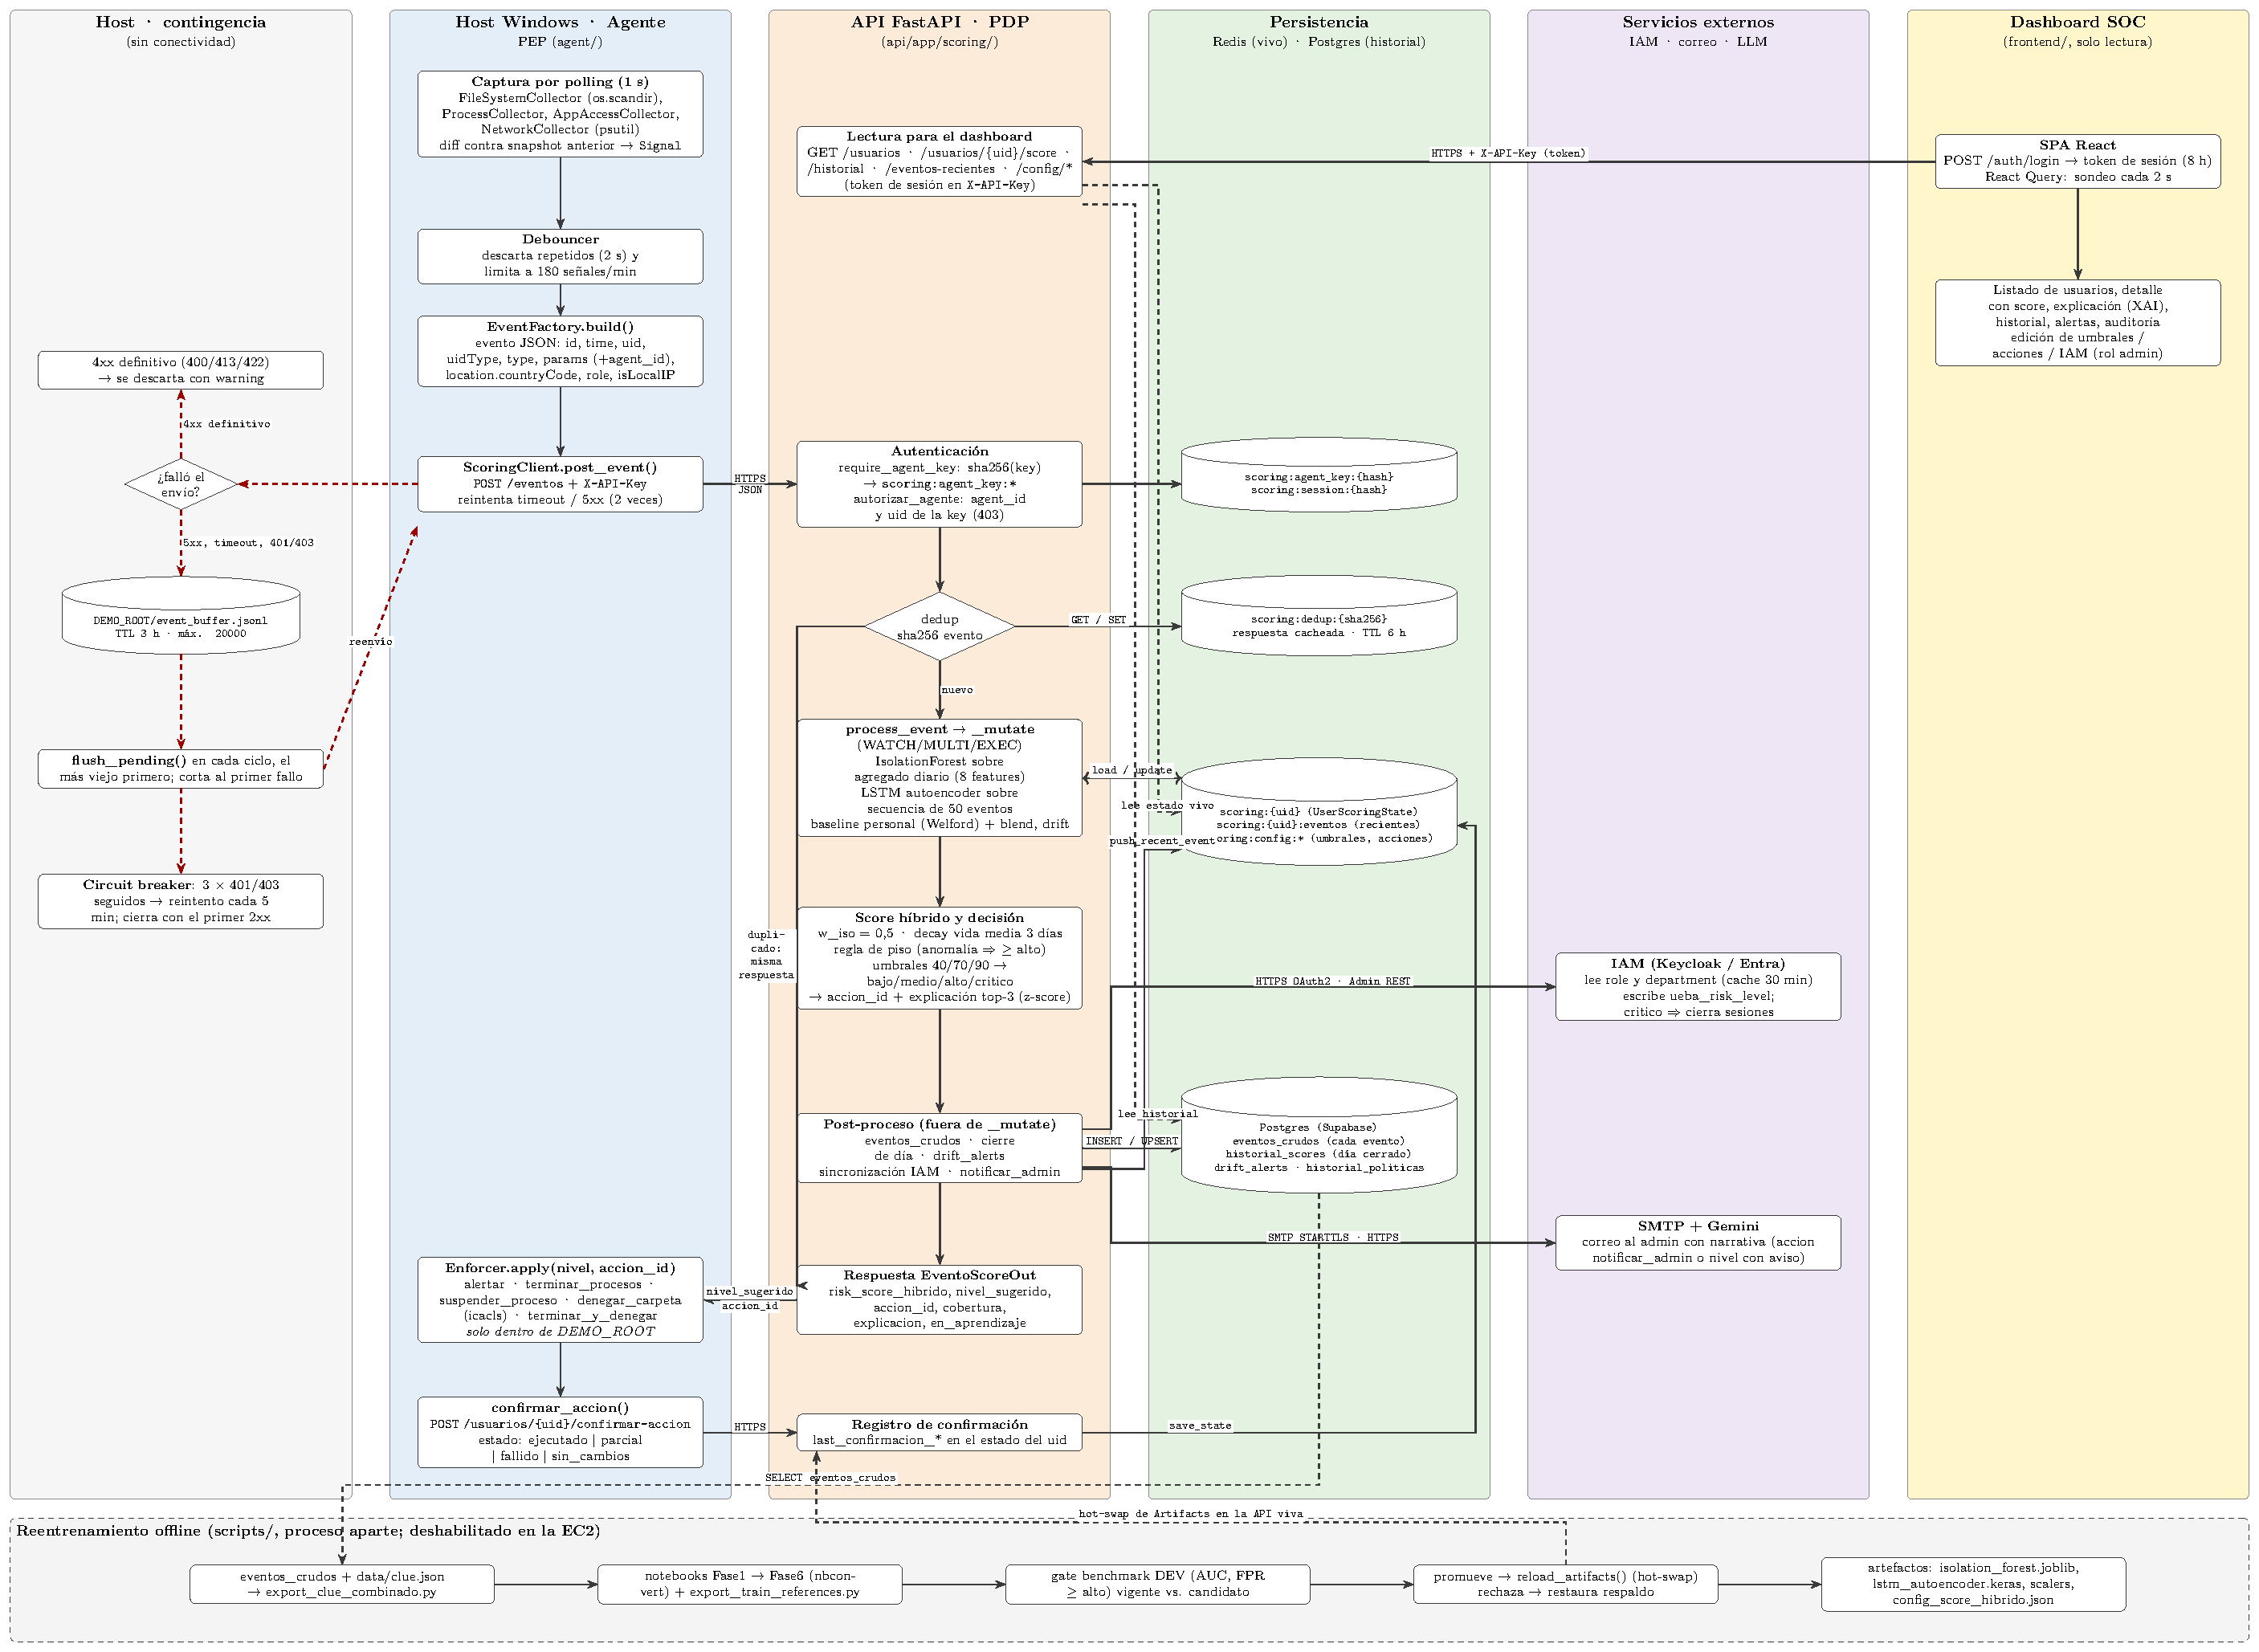
\includegraphics[trim=0bp 0bp 675.15bp 0bp, clip, width=\textwidth, height=0.84\textheight, keepaspectratio]{images/diagramas/uml/01_flujo_informacion.pdf}
    \caption{Diagrama de flujo de información del sistema, versión completa (mitad izquierda)}
    \label{fig:anexo-flujo-izq}
    {\small Fuente: elaboración propia.\par}
\end{figure}
\clearpage

\begin{figure}[p]
    \centering
    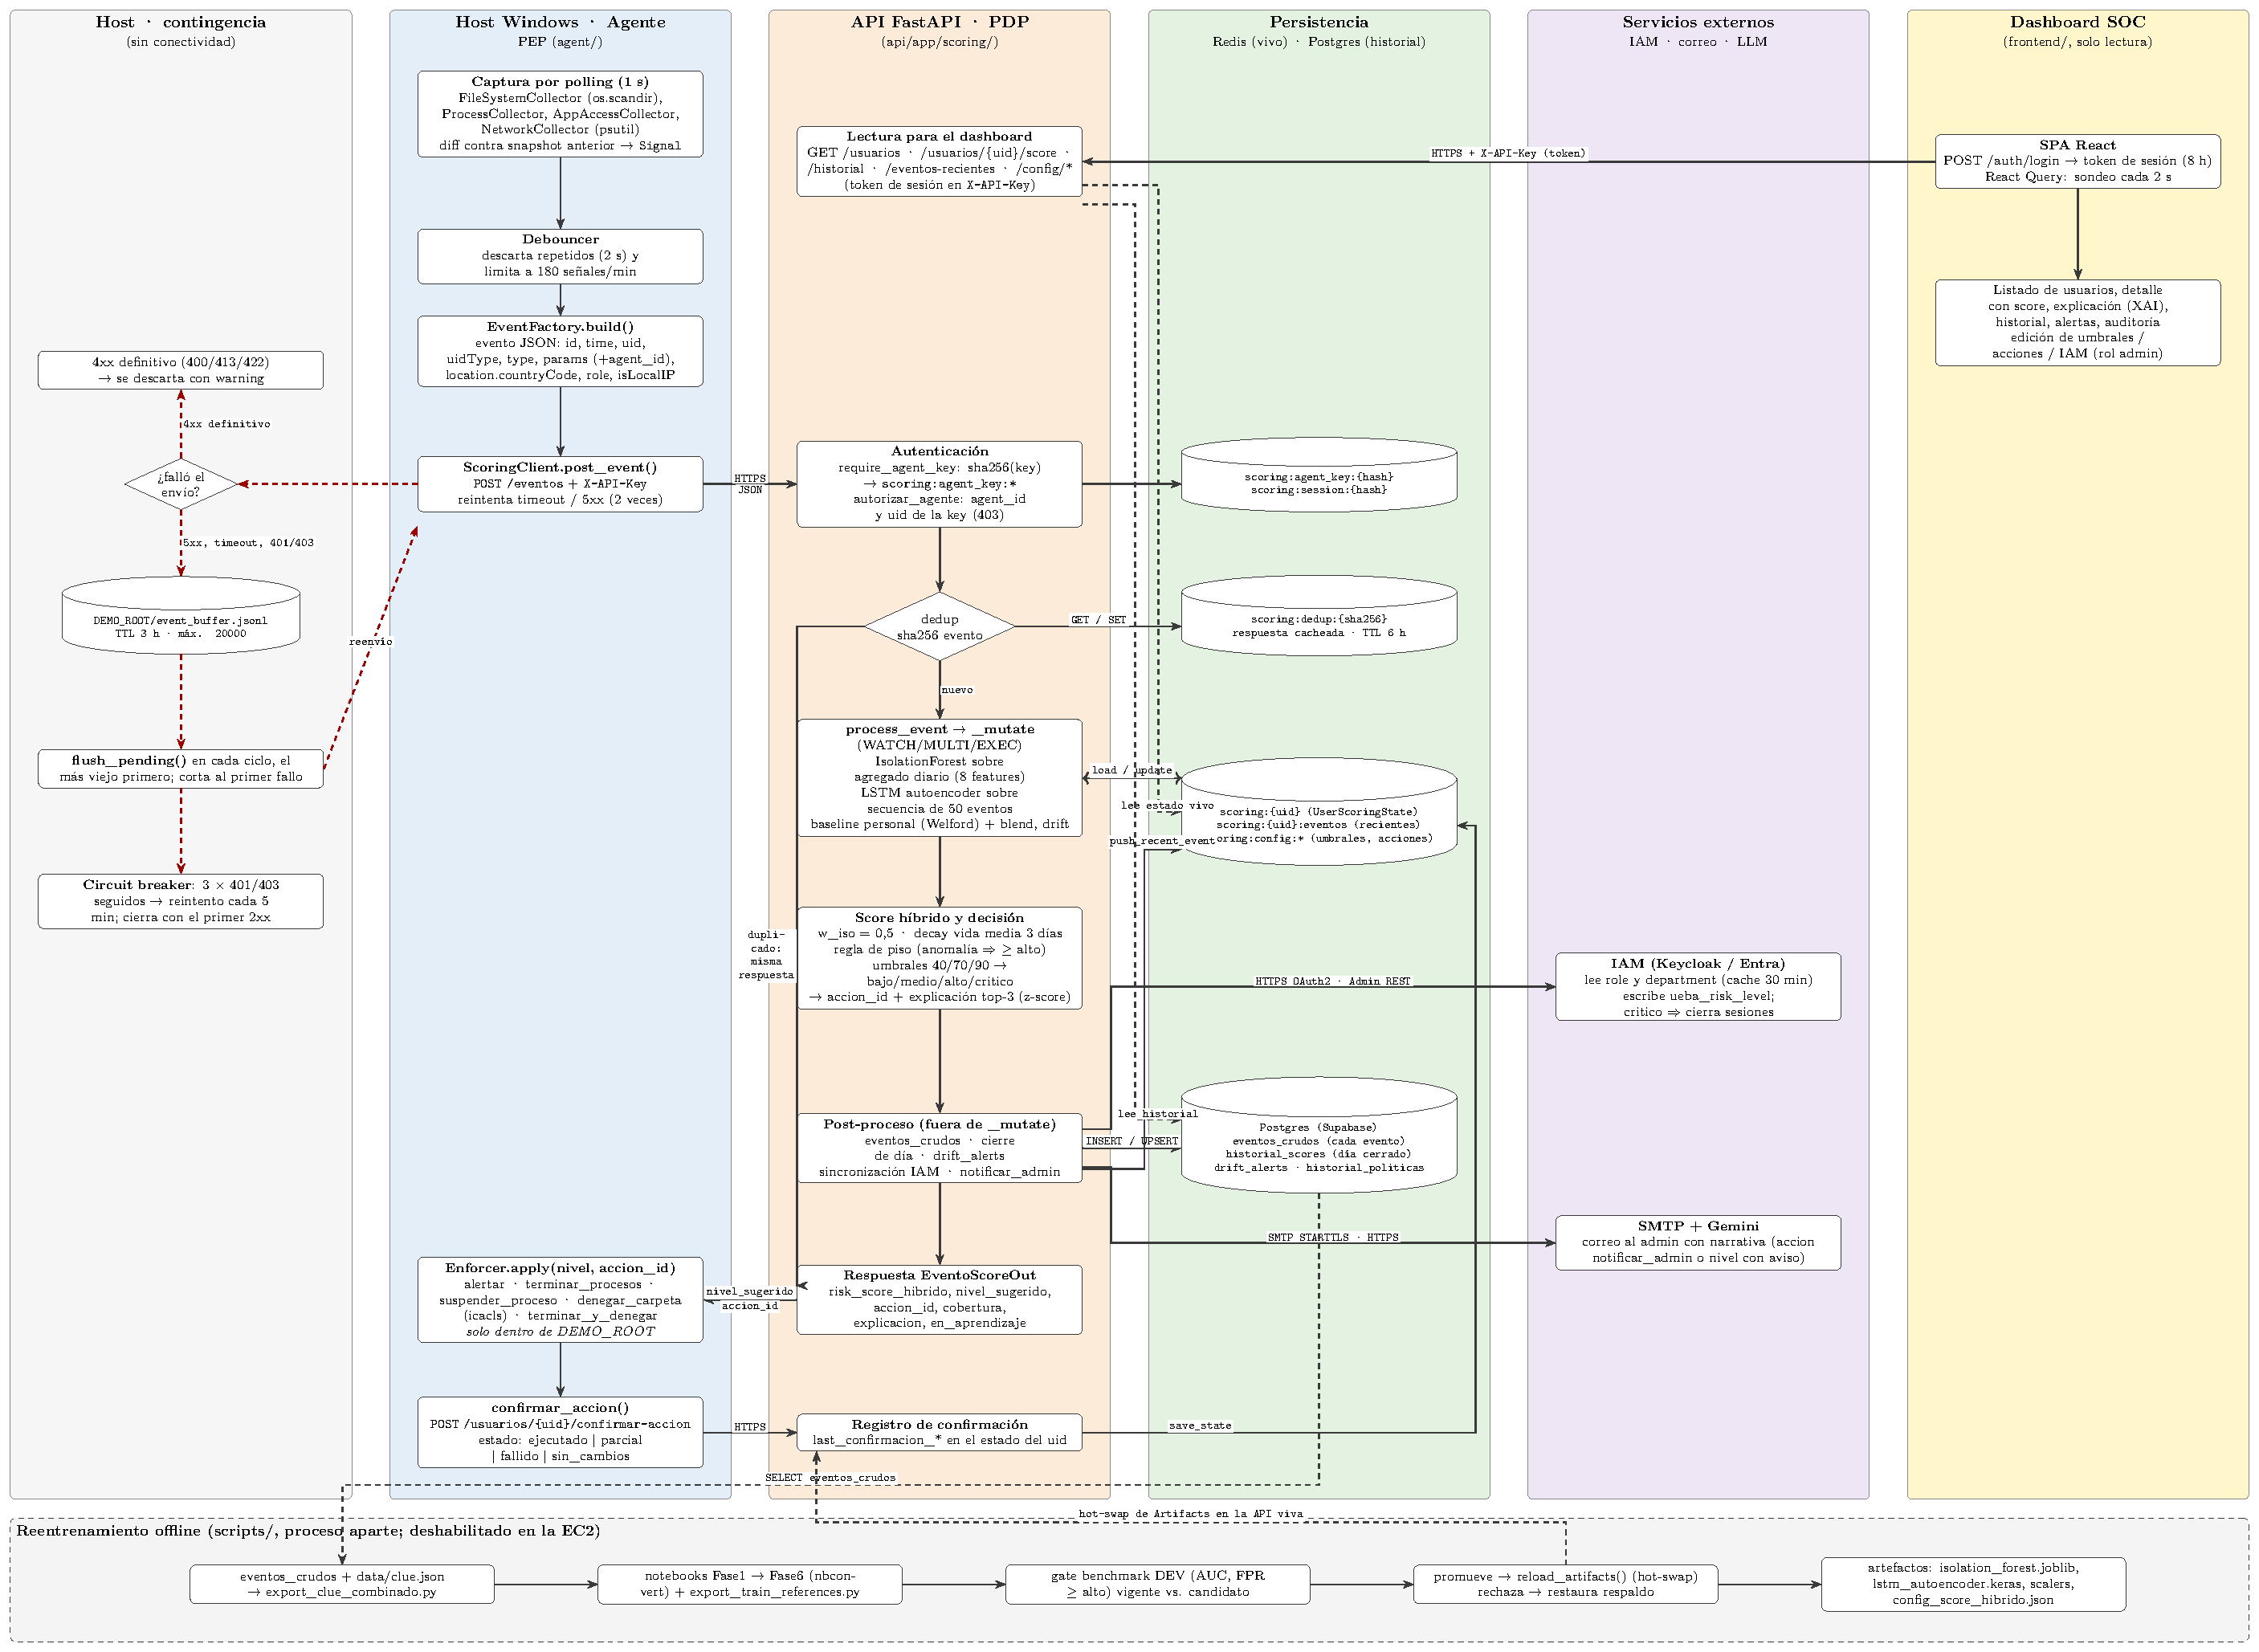
\includegraphics[trim=675.15bp 0bp 0bp 0bp, clip, width=\textwidth, height=0.84\textheight, keepaspectratio]{images/diagramas/uml/01_flujo_informacion.pdf}
    \caption{Diagrama de flujo de información del sistema, versión completa (mitad derecha)}
    \label{fig:anexo-flujo-der}
    {\small Fuente: elaboración propia.\par}
\end{figure}
\clearpage

\begin{figure}[p]
    \centering
    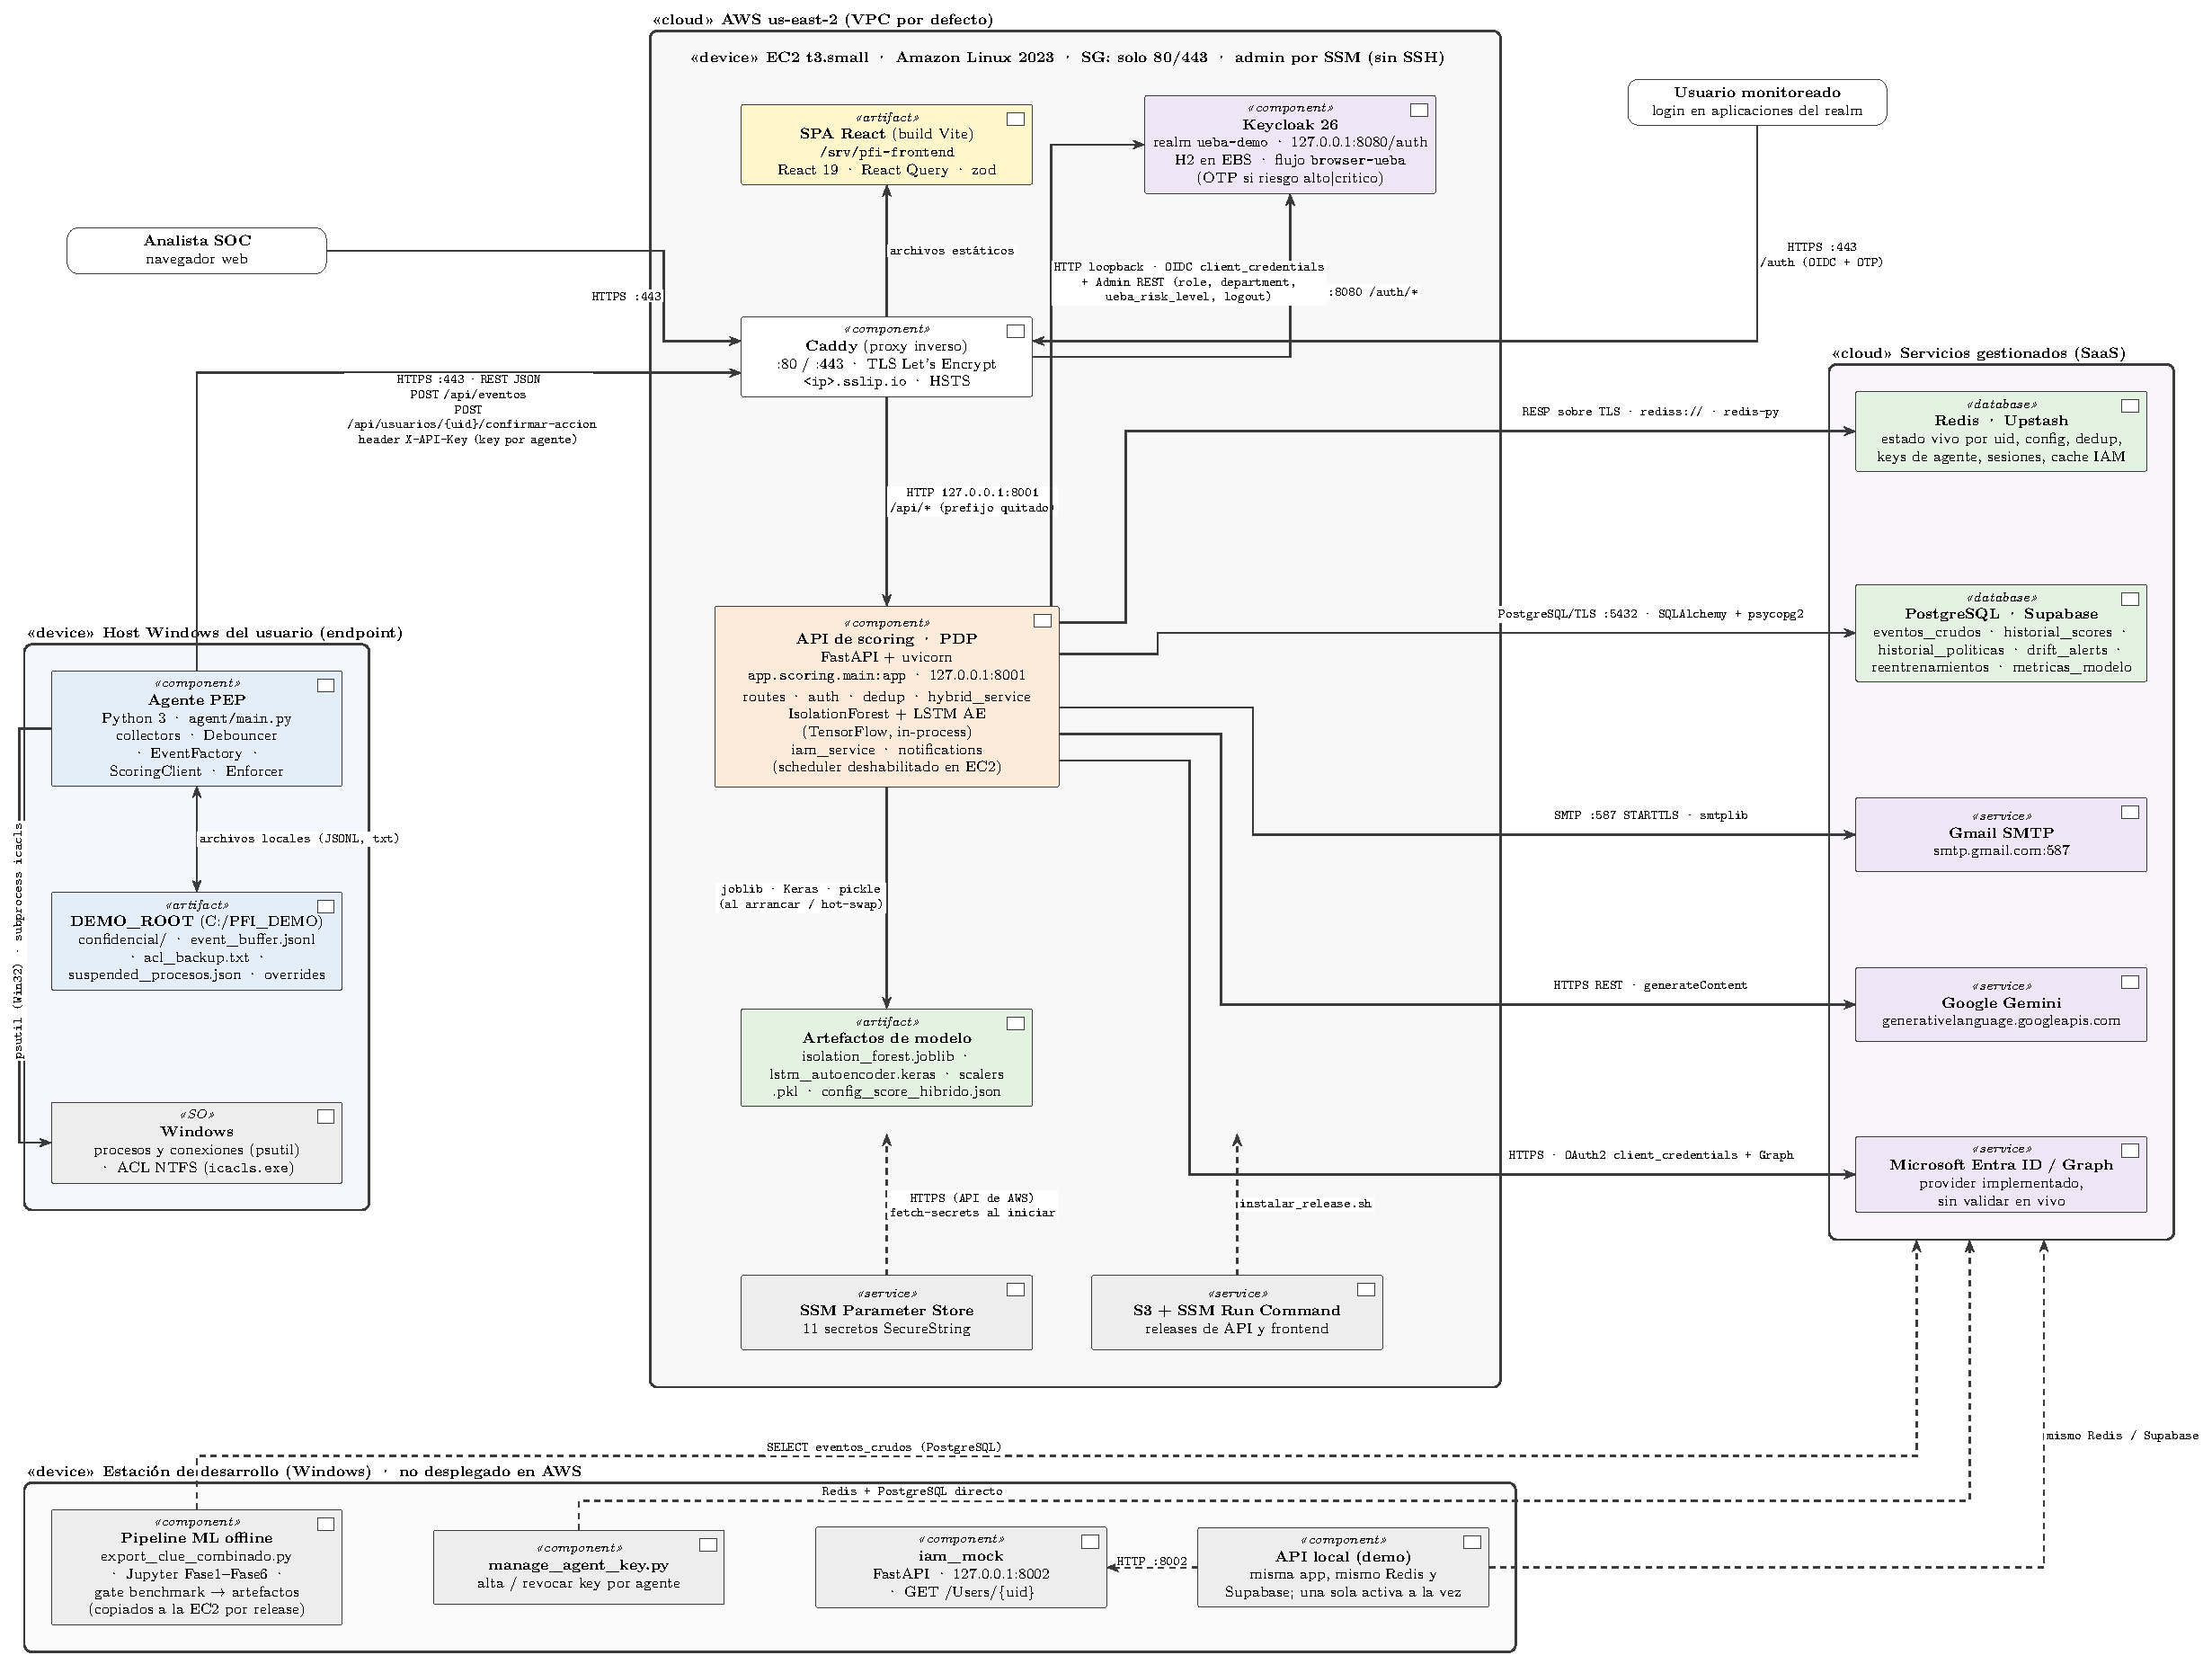
\includegraphics[trim=0bp 0bp 590.72bp 0bp, clip, width=\textwidth, height=0.84\textheight, keepaspectratio]{images/diagramas/uml/02_componentes_protocolos.pdf}
    \caption{Diagrama de componentes con protocolos de comunicación, versión completa (mitad izquierda)}
    \label{fig:anexo-componentes-izq}
    {\small Fuente: elaboración propia.\par}
\end{figure}
\clearpage

\begin{figure}[p]
    \centering
    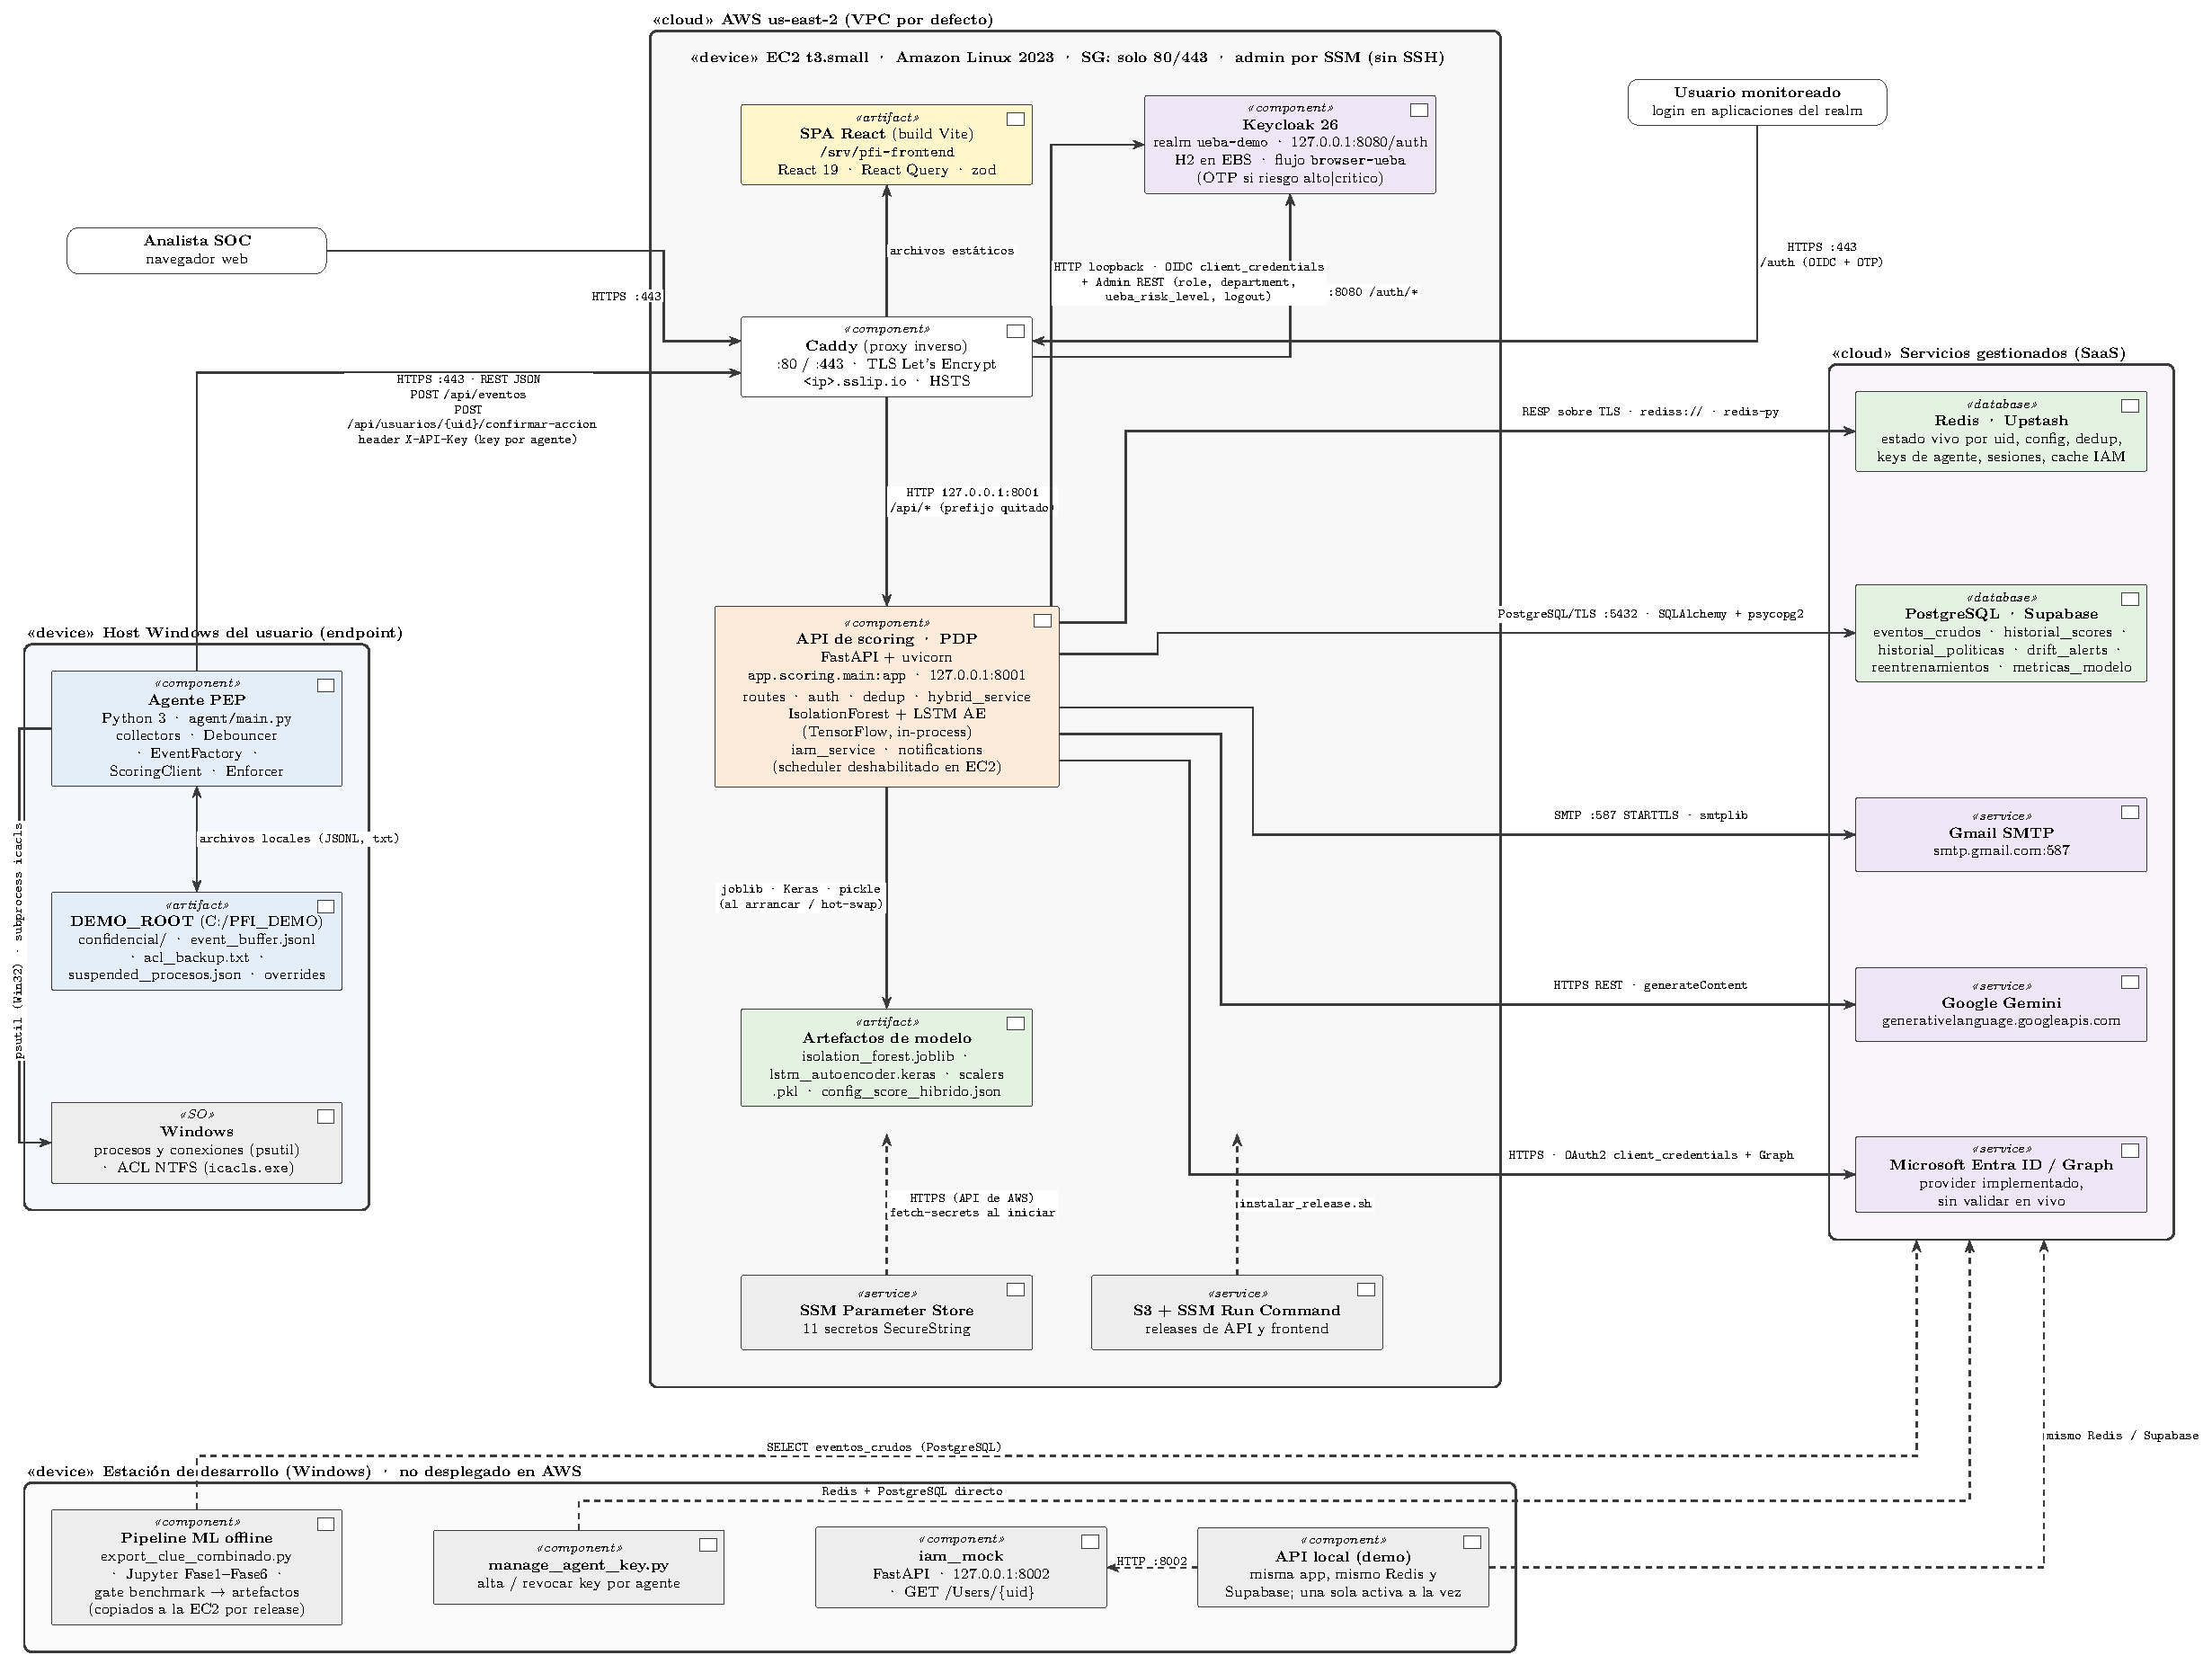
\includegraphics[trim=590.72bp 0bp 0bp 0bp, clip, width=\textwidth, height=0.84\textheight, keepaspectratio]{images/diagramas/uml/02_componentes_protocolos.pdf}
    \caption{Diagrama de componentes con protocolos de comunicación, versión completa (mitad derecha)}
    \label{fig:anexo-componentes-der}
    {\small Fuente: elaboración propia.\par}
\end{figure}
\clearpage

\begin{figure}[p]
    \centering
    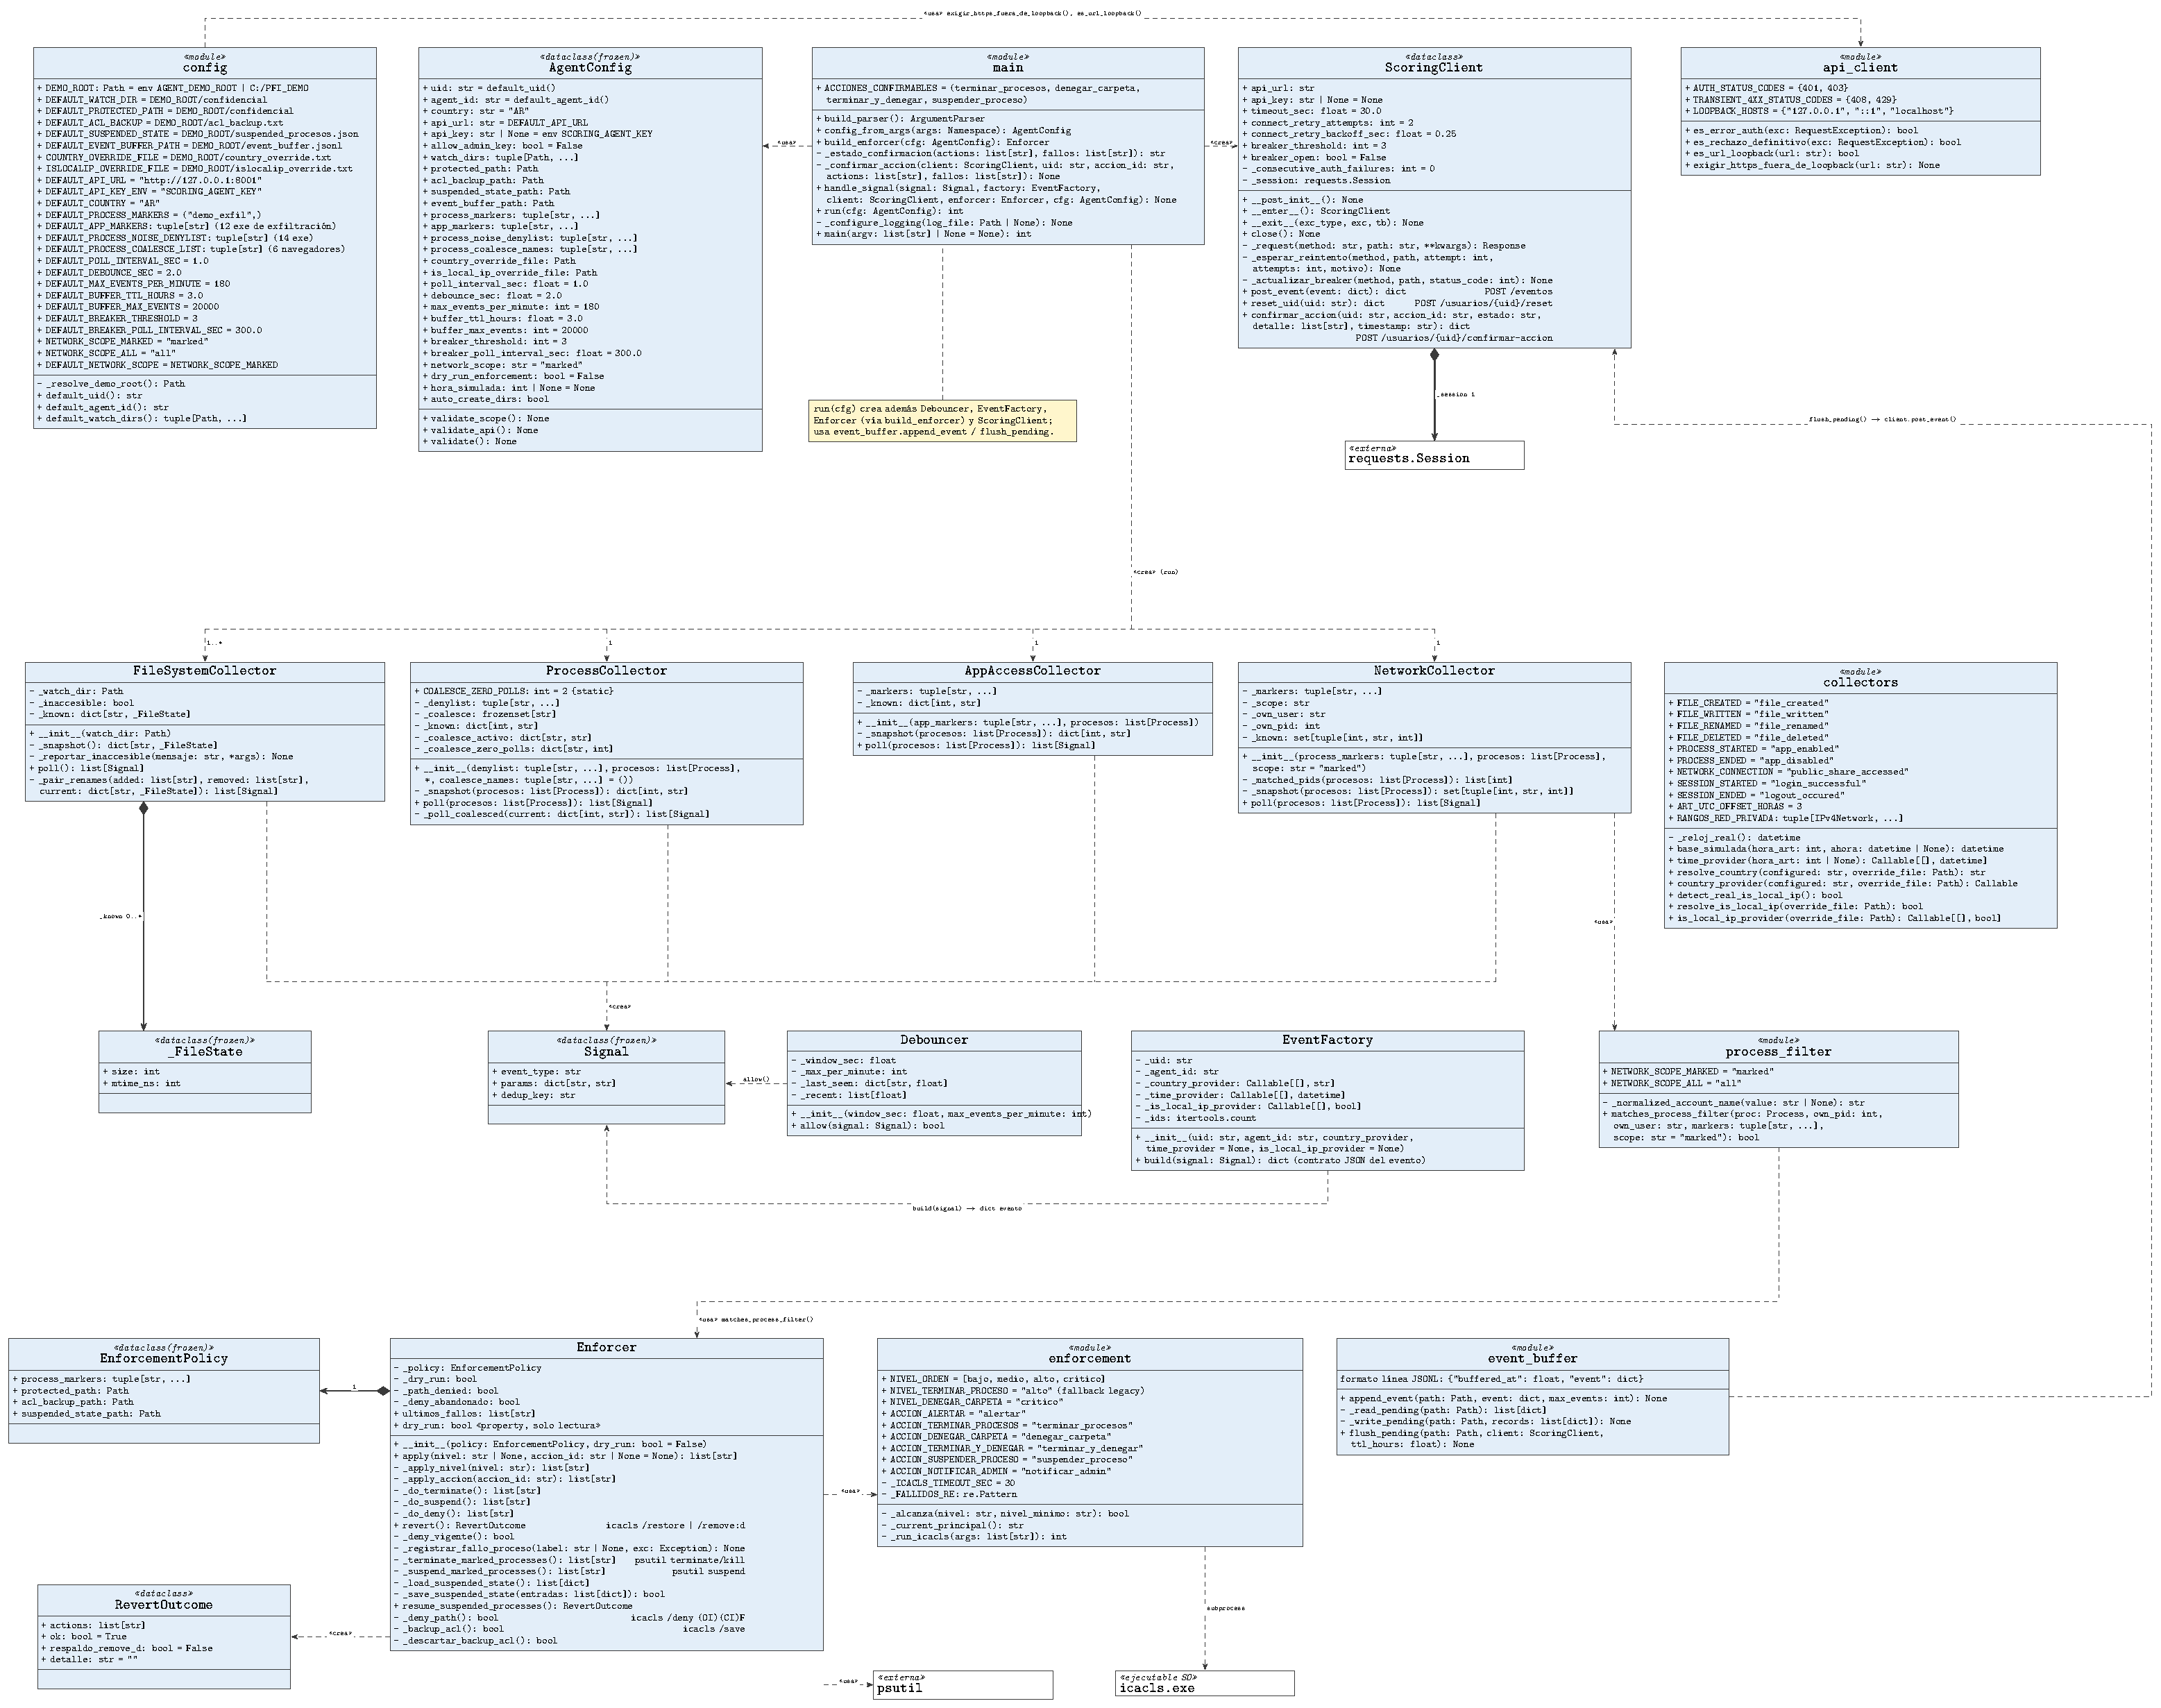
\includegraphics[trim=0bp 0bp 747.26bp 0bp, clip, width=\textwidth, height=0.84\textheight, keepaspectratio]{images/diagramas/uml/03_clases_agente_pep.pdf}
    \caption{Diagrama de clases del agente PEP, versión completa (mitad izquierda)}
    \label{fig:anexo-clases-agente-izq}
    {\small Fuente: elaboración propia.\par}
\end{figure}
\clearpage

\begin{figure}[p]
    \centering
    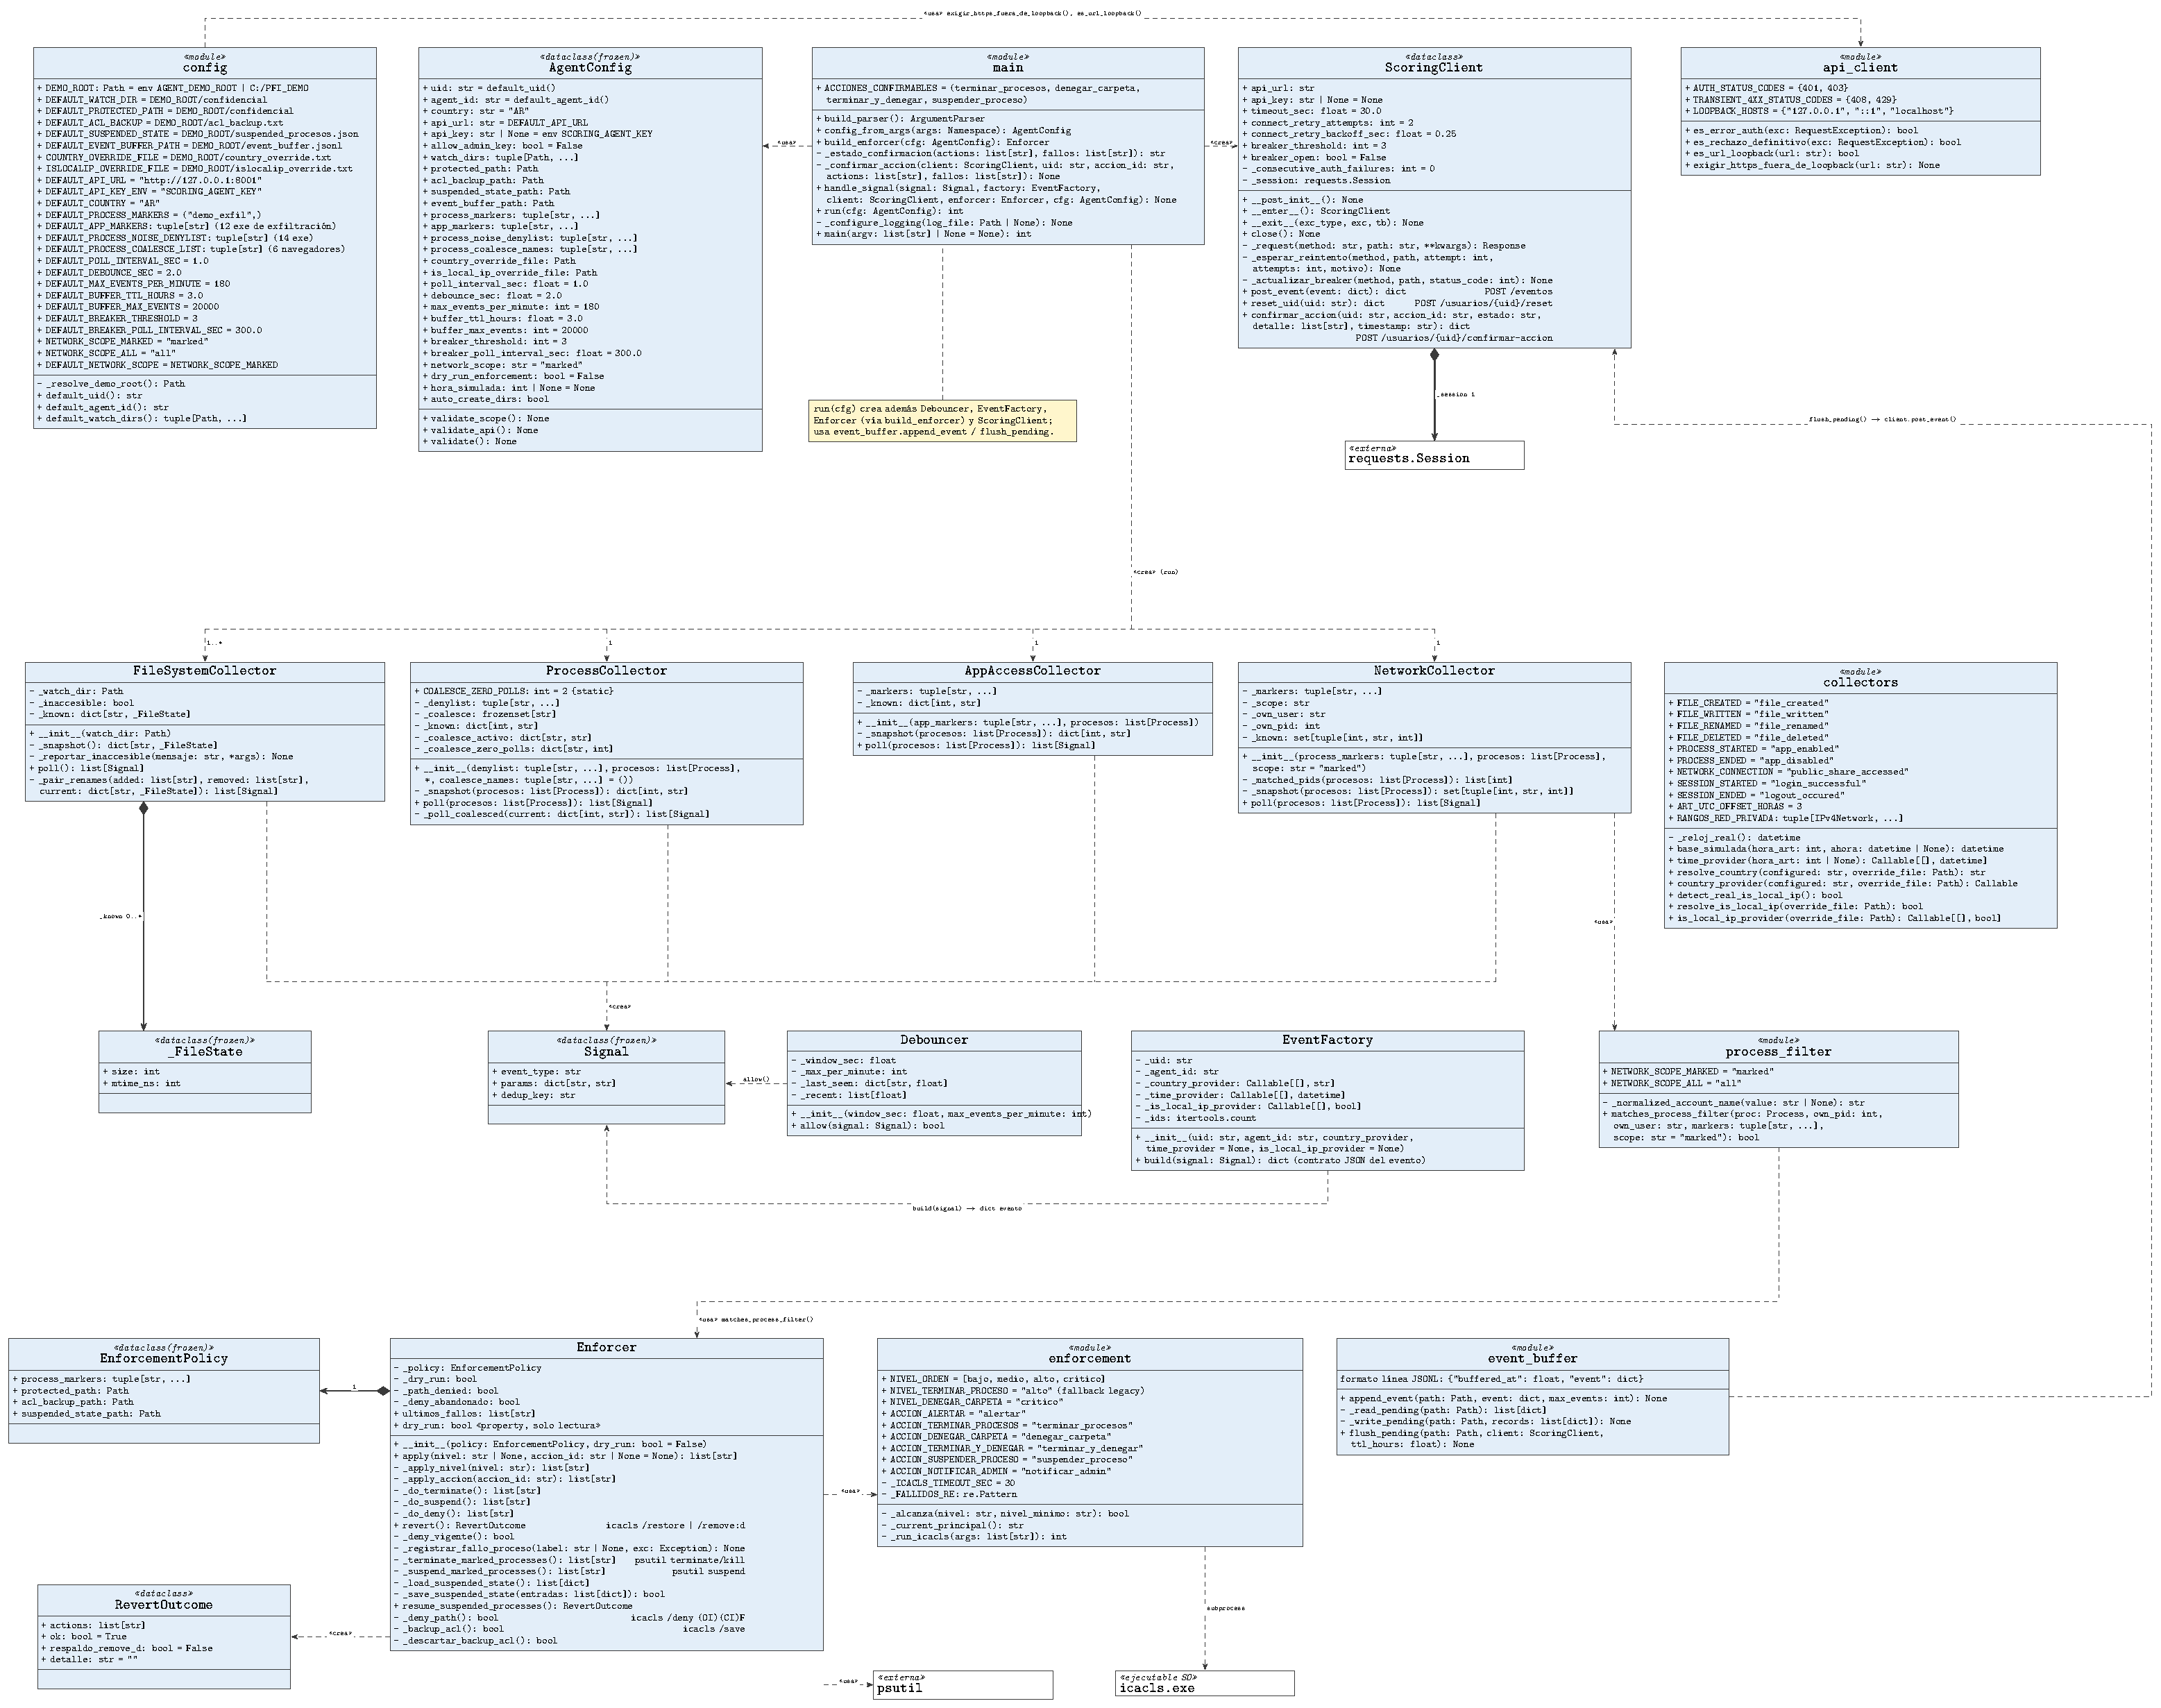
\includegraphics[trim=747.26bp 0bp 0bp 0bp, clip, width=\textwidth, height=0.84\textheight, keepaspectratio]{images/diagramas/uml/03_clases_agente_pep.pdf}
    \caption{Diagrama de clases del agente PEP, versión completa (mitad derecha)}
    \label{fig:anexo-clases-agente-der}
    {\small Fuente: elaboración propia.\par}
\end{figure}
\clearpage

\begin{figure}[p]
    \centering
    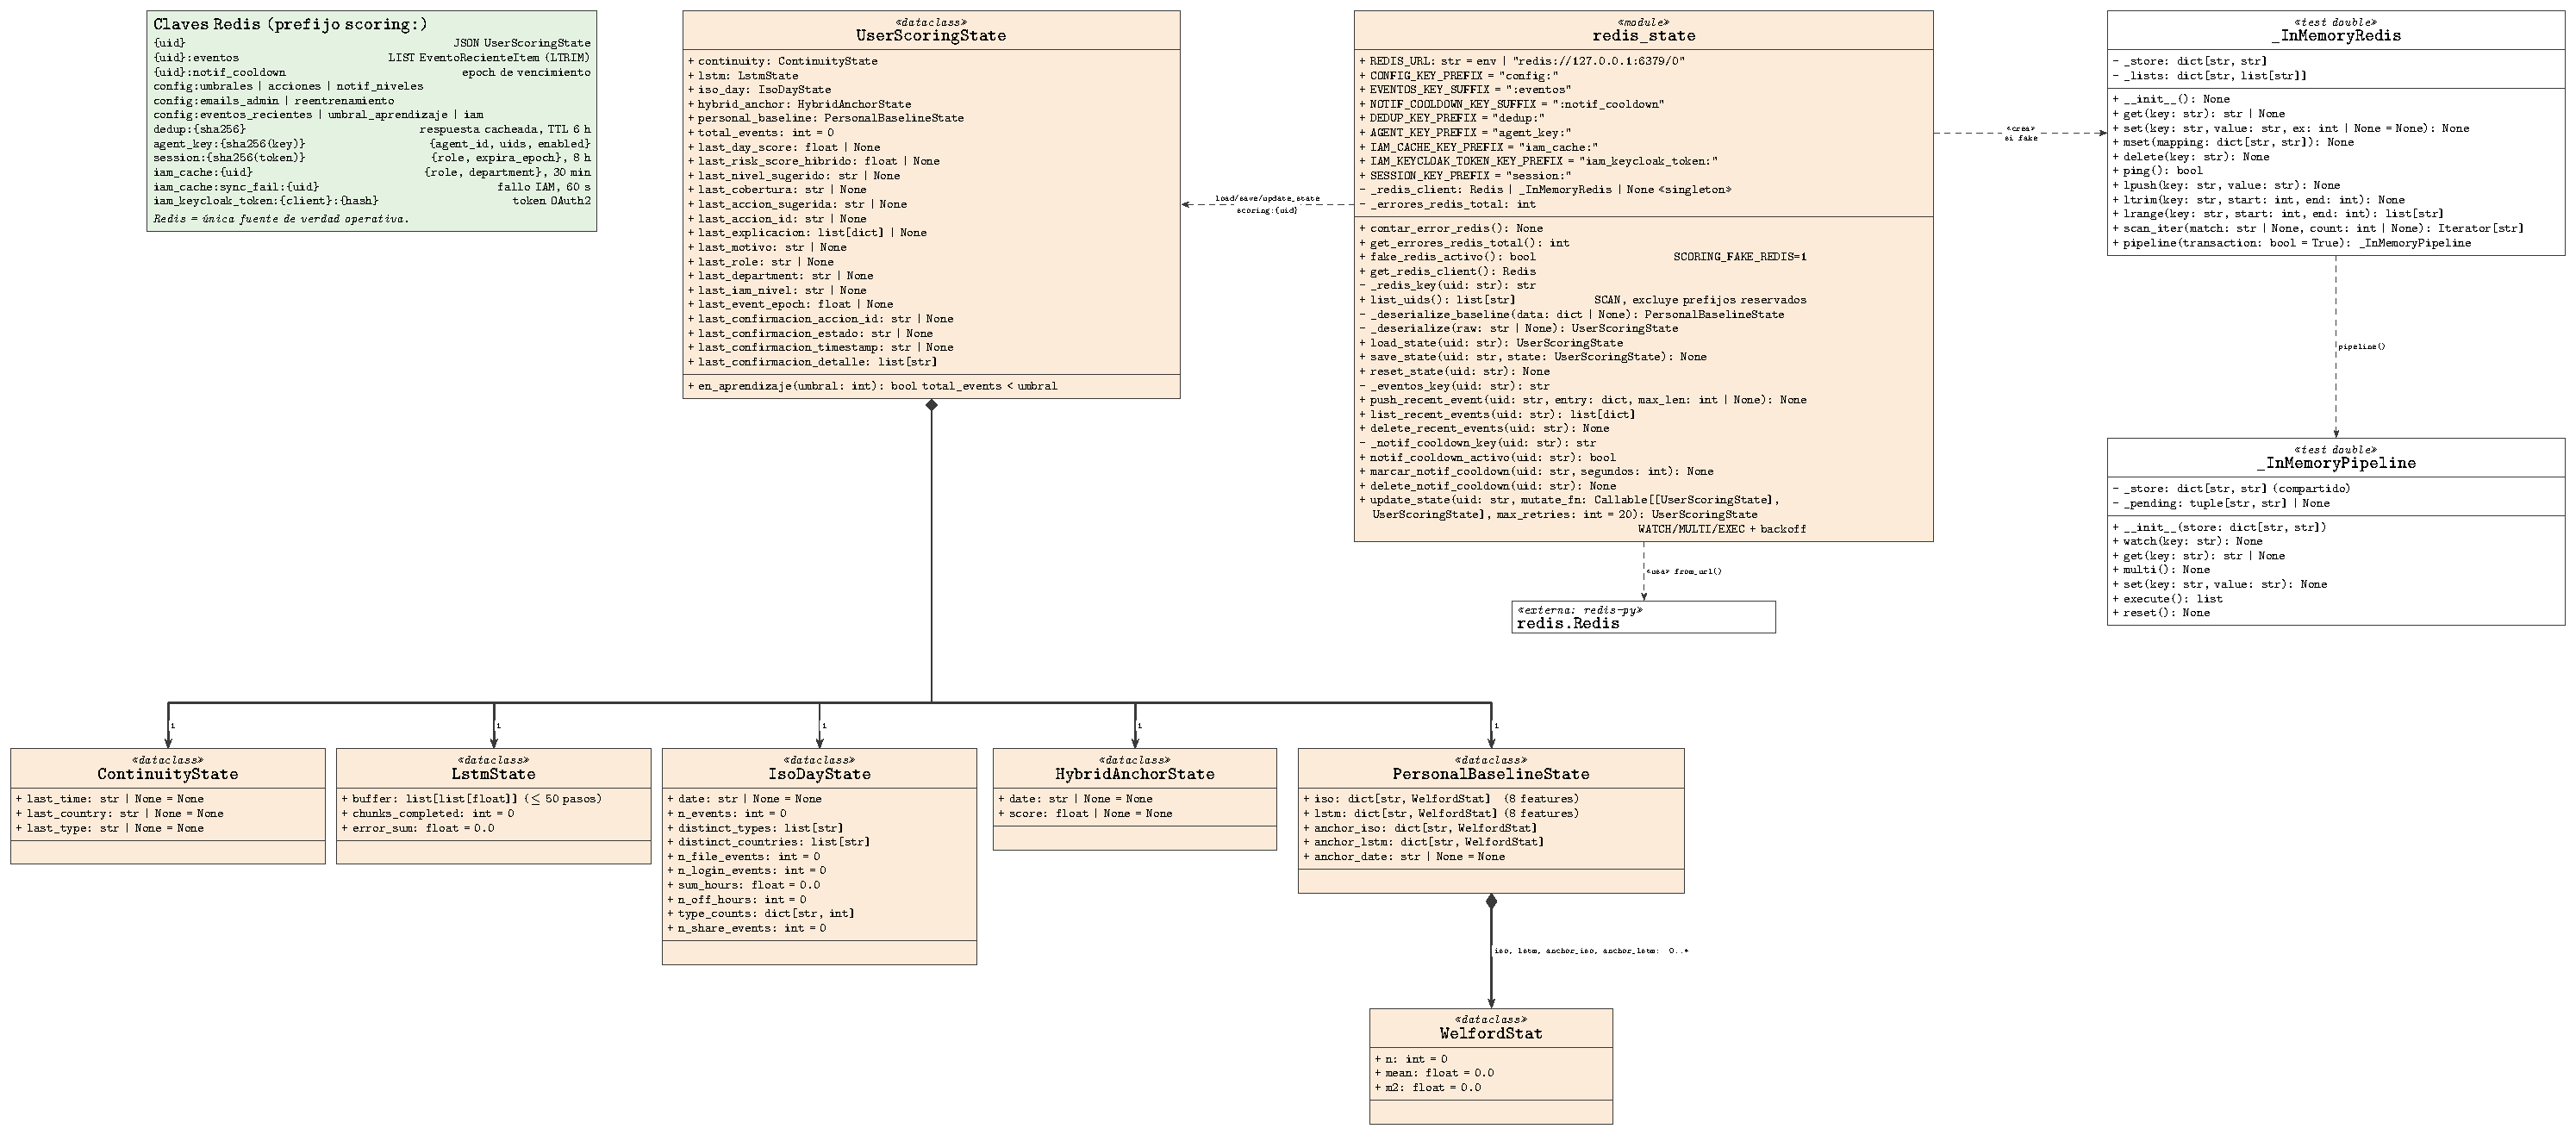
\includegraphics[trim=0bp 0bp 717.33bp 0bp, clip, width=\textwidth, height=0.84\textheight, keepaspectratio]{images/diagramas/uml/04a_clases_api_estado.pdf}
    \caption{Diagrama de clases de la API PDP: estado del usuario en Redis, versión completa (mitad izquierda)}
    \label{fig:anexo-clases-redis-izq}
    {\small Fuente: elaboración propia.\par}
\end{figure}
\clearpage

\begin{figure}[p]
    \centering
    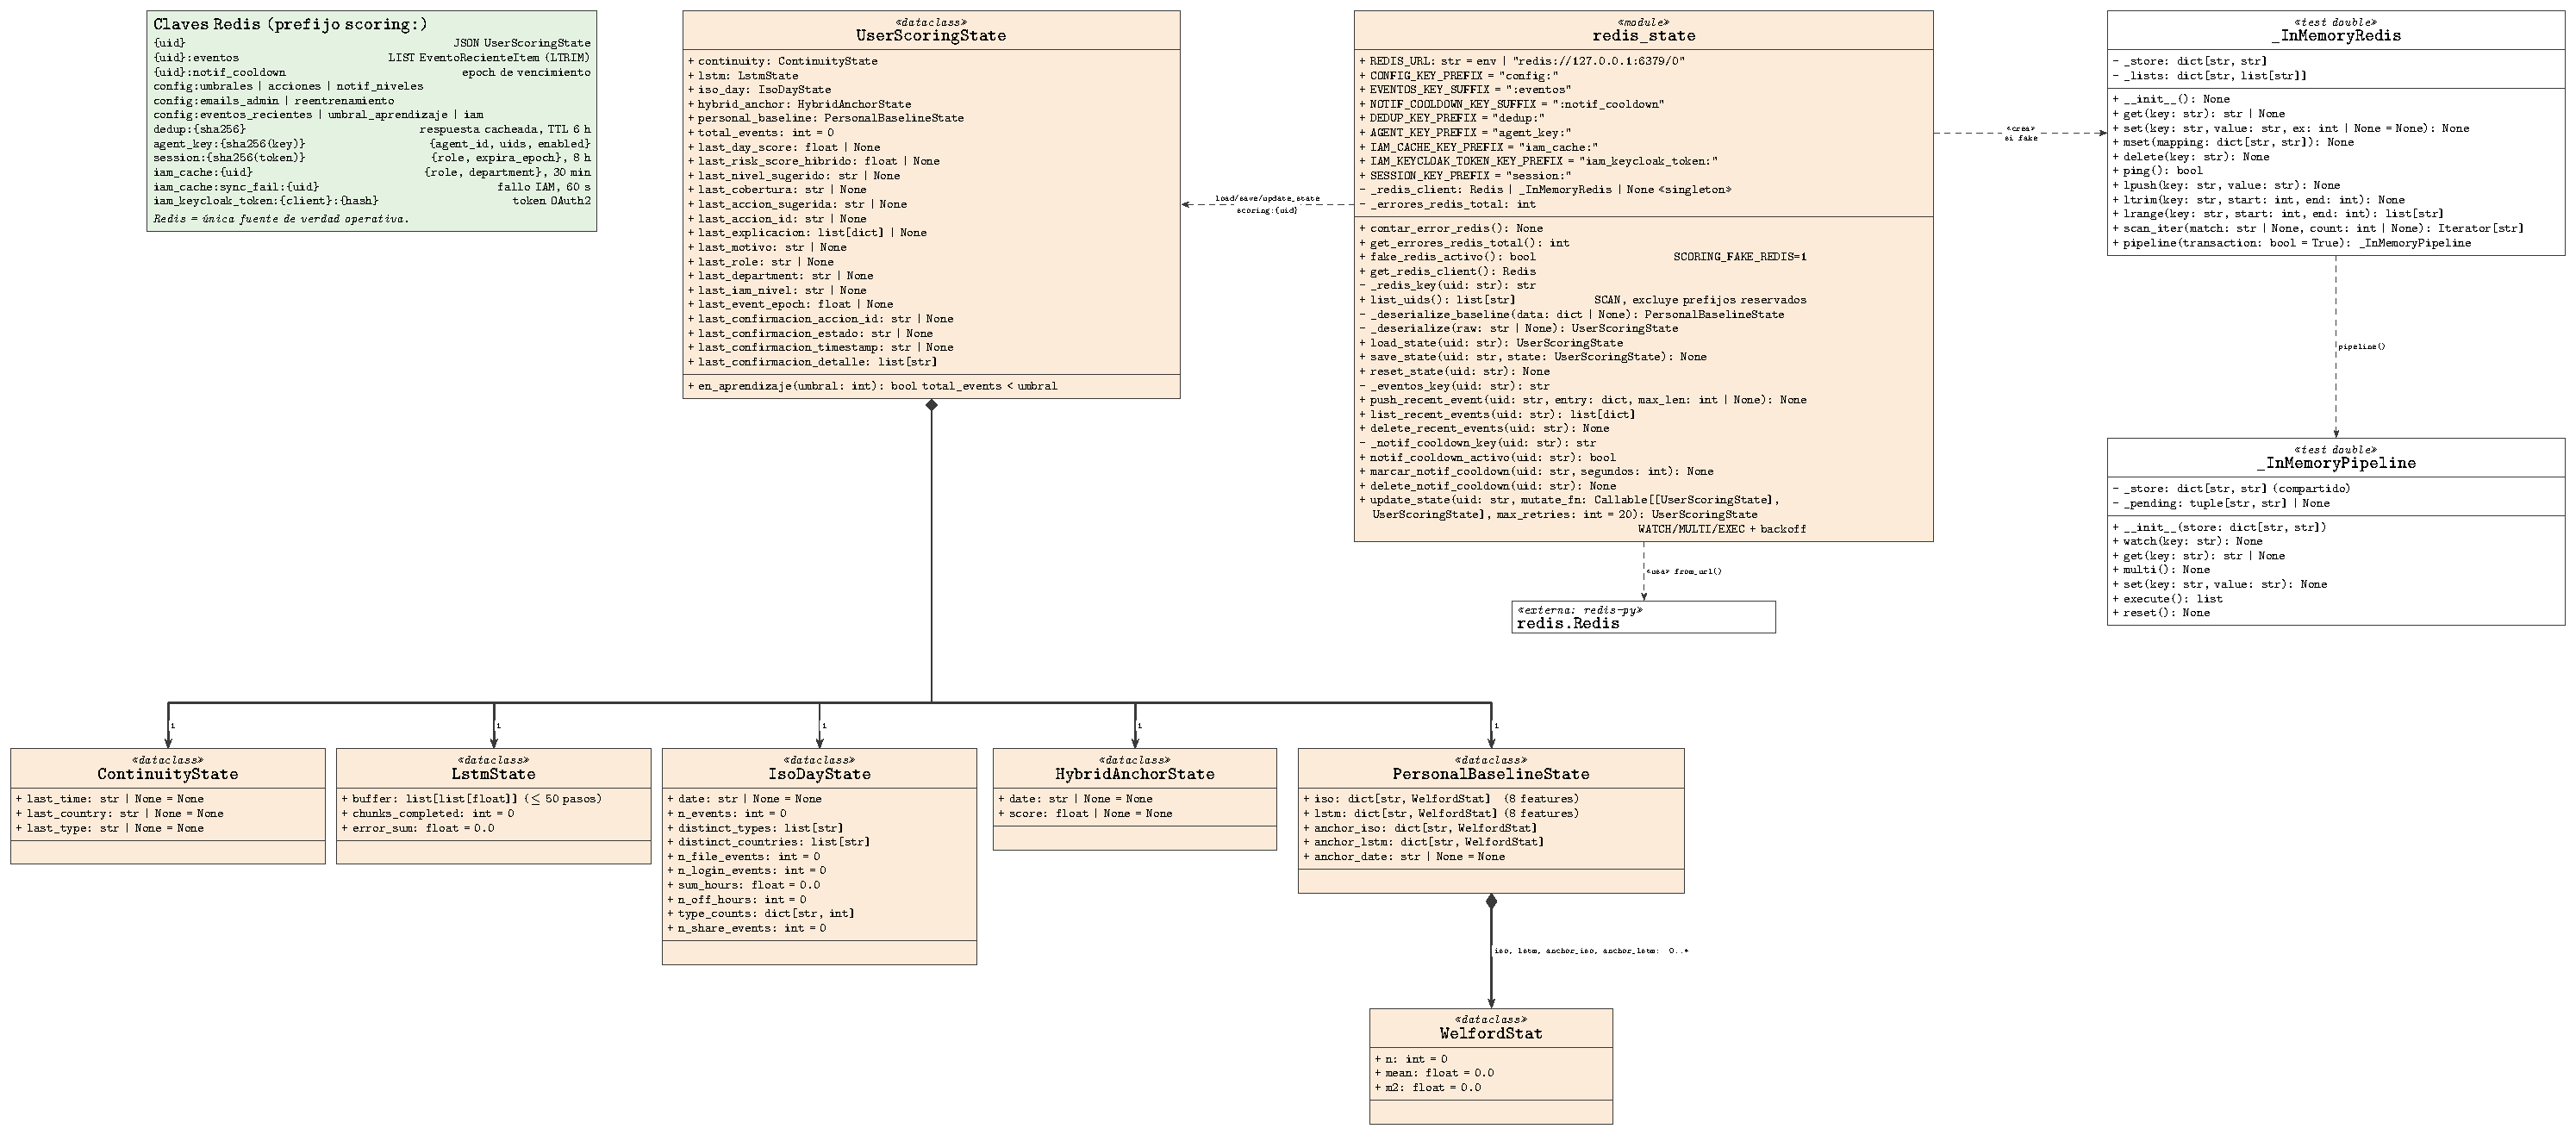
\includegraphics[trim=717.33bp 0bp 0bp 0bp, clip, width=\textwidth, height=0.84\textheight, keepaspectratio]{images/diagramas/uml/04a_clases_api_estado.pdf}
    \caption{Diagrama de clases de la API PDP: estado del usuario en Redis, versión completa (mitad derecha)}
    \label{fig:anexo-clases-redis-der}
    {\small Fuente: elaboración propia.\par}
\end{figure}
\clearpage

\begin{figure}[p]
    \centering
    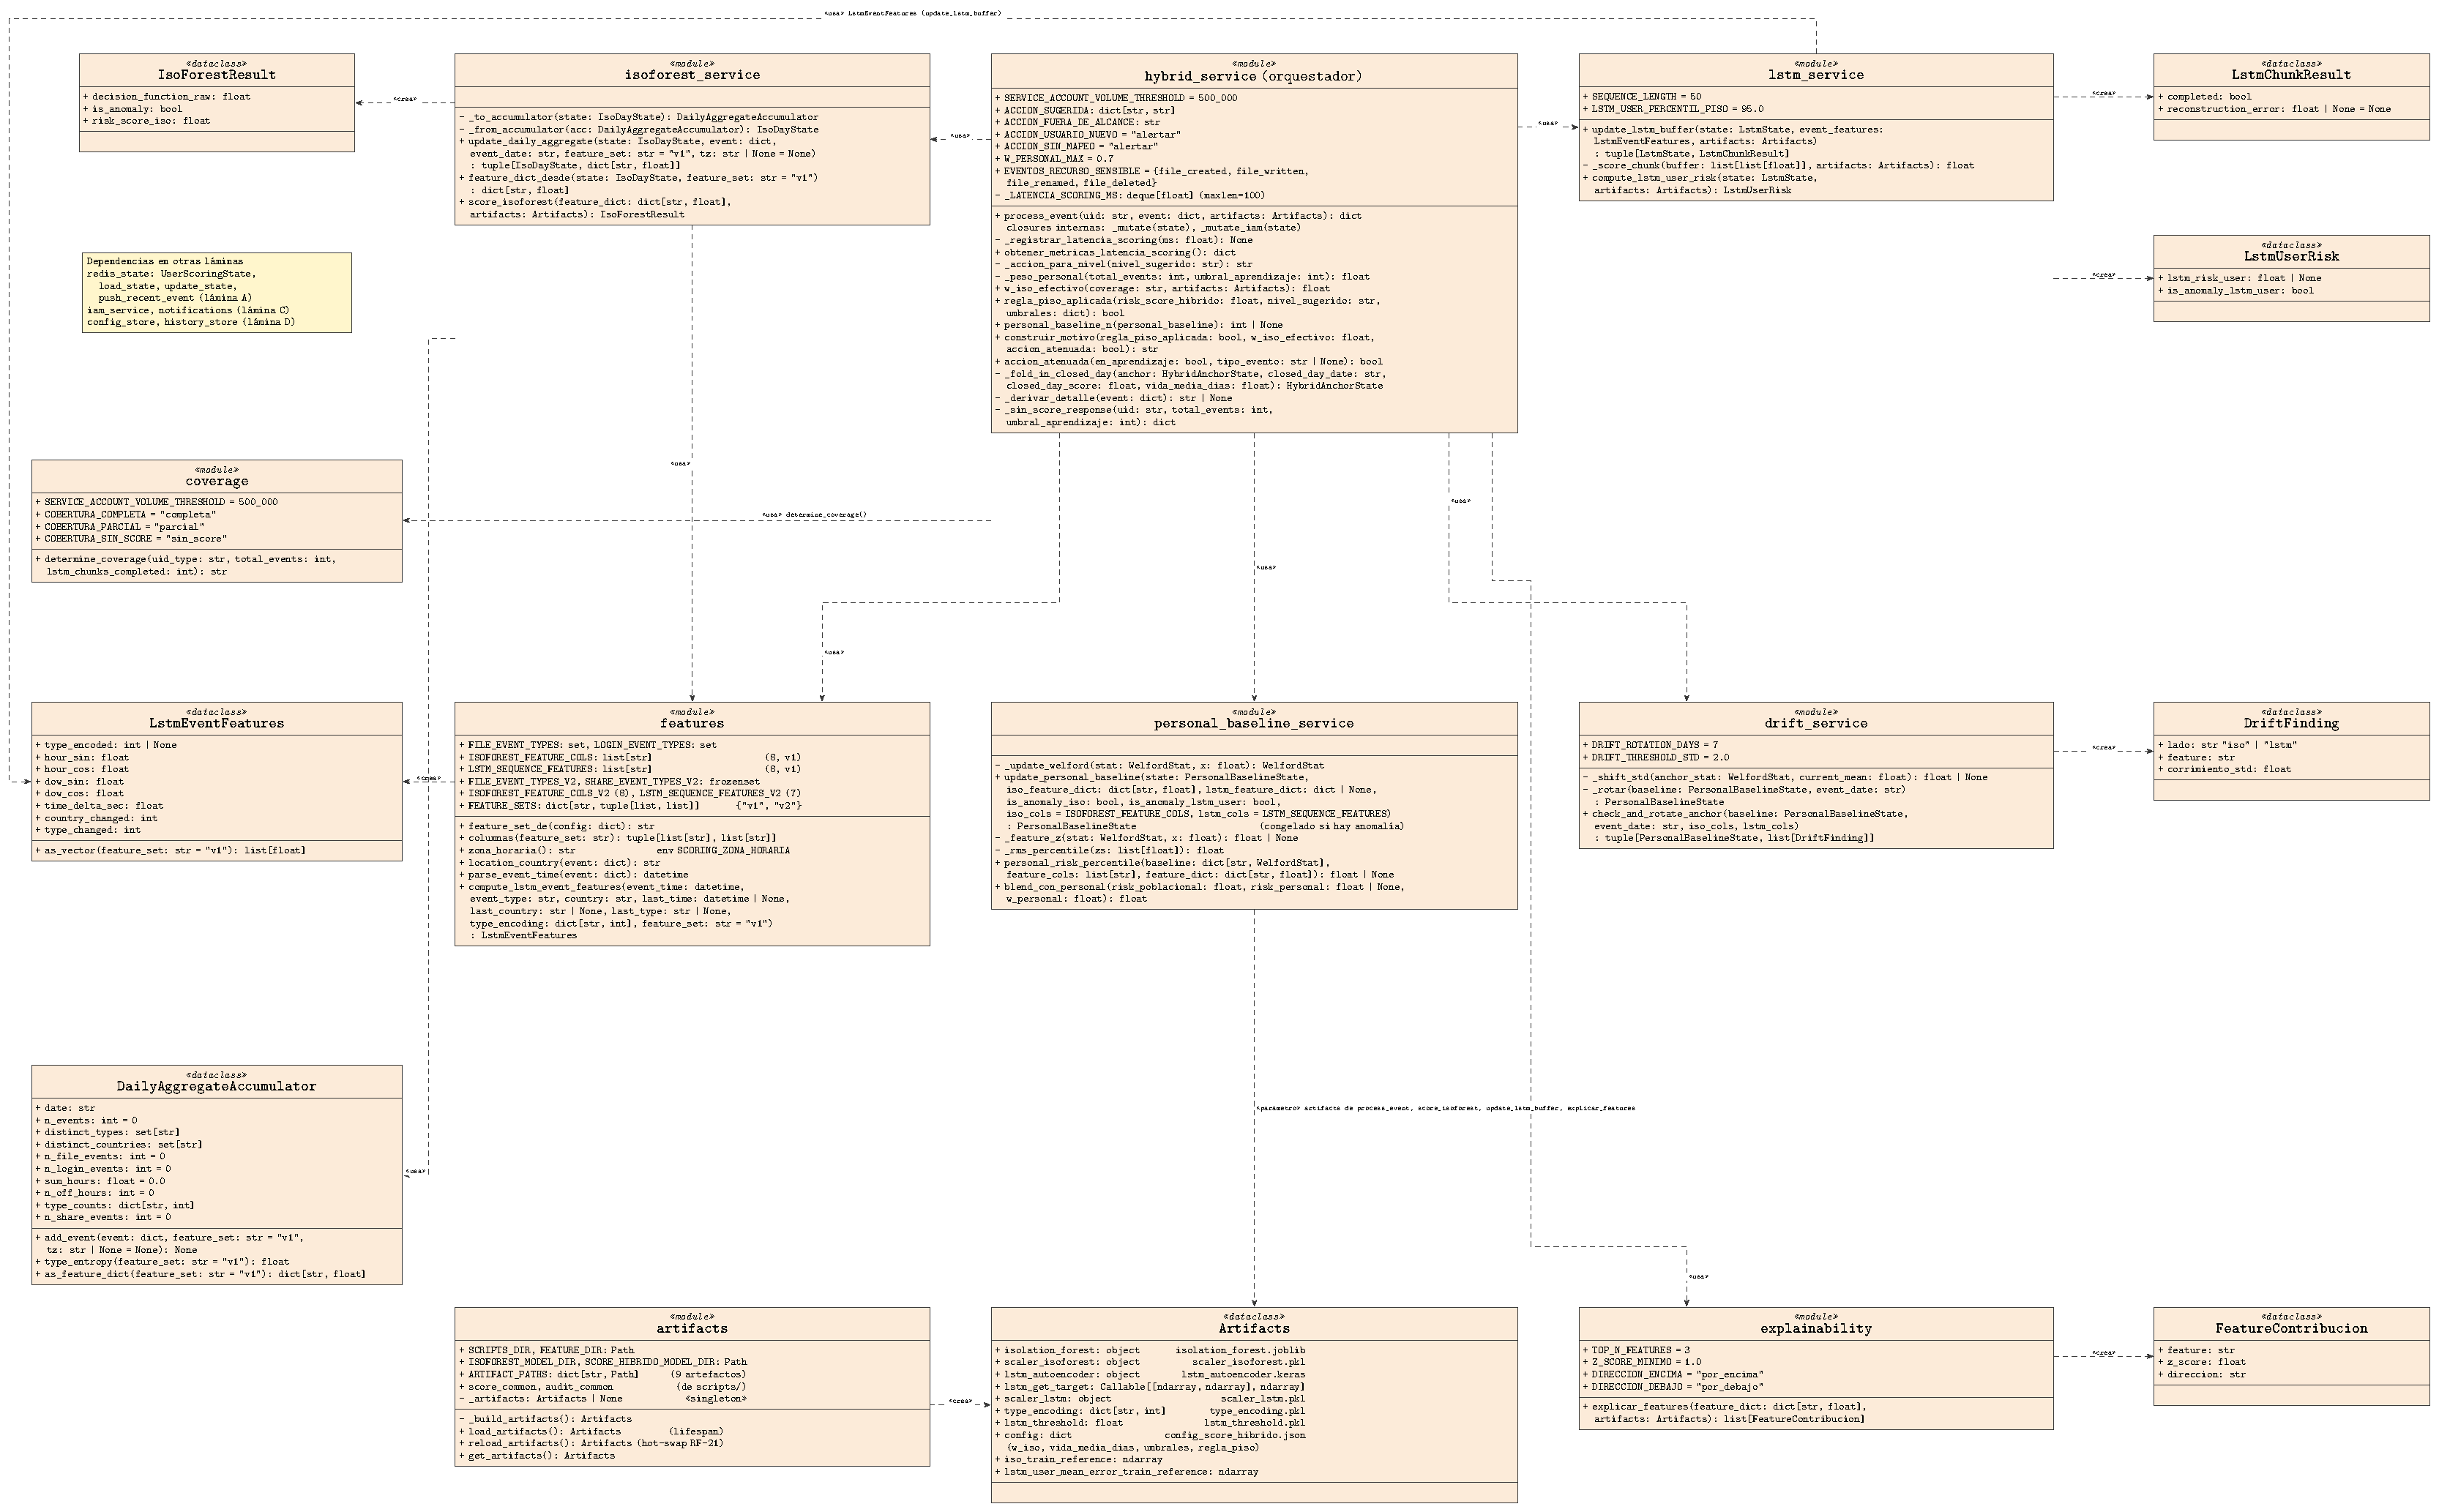
\includegraphics[trim=0bp 0bp 799.71bp 0bp, clip, width=\textwidth, height=0.84\textheight, keepaspectratio]{images/diagramas/uml/04b_clases_api_scoring.pdf}
    \caption{Diagrama de clases de la API PDP: puntaje y modelos, versión completa (mitad izquierda)}
    \label{fig:anexo-clases-scoring-izq}
    {\small Fuente: elaboración propia.\par}
\end{figure}
\clearpage

\begin{figure}[p]
    \centering
    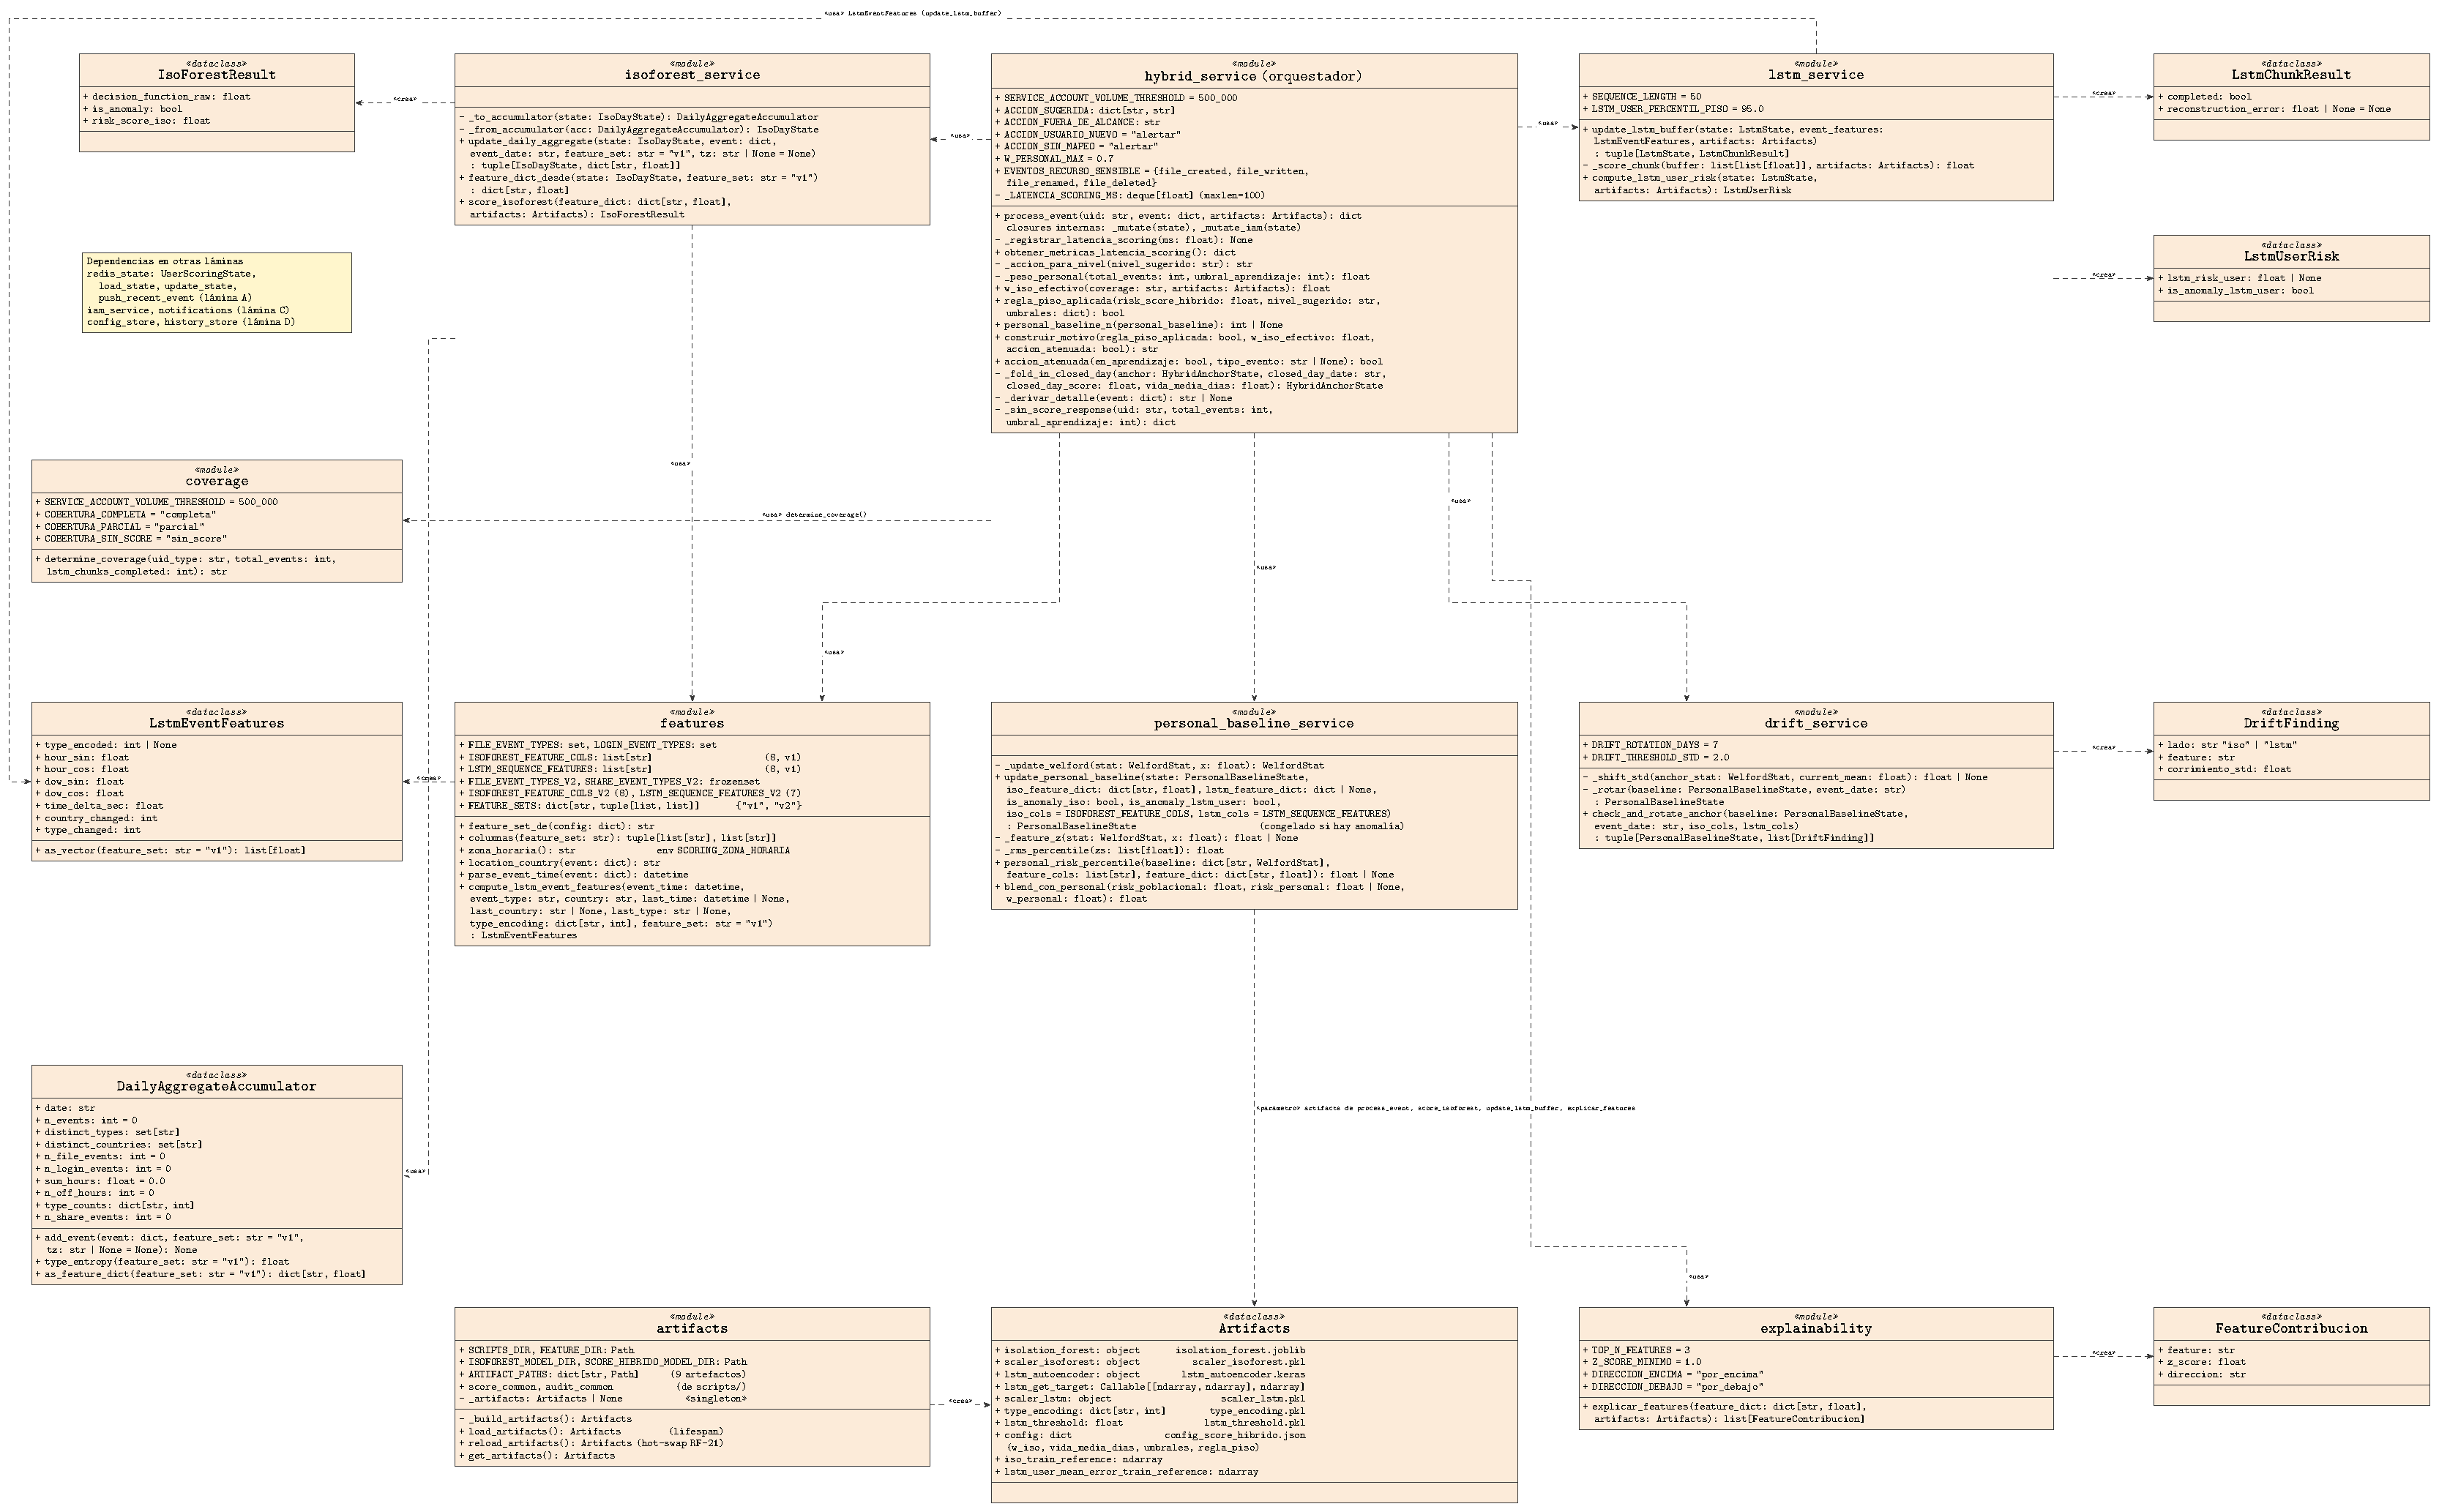
\includegraphics[trim=799.71bp 0bp 0bp 0bp, clip, width=\textwidth, height=0.84\textheight, keepaspectratio]{images/diagramas/uml/04b_clases_api_scoring.pdf}
    \caption{Diagrama de clases de la API PDP: puntaje y modelos, versión completa (mitad derecha)}
    \label{fig:anexo-clases-scoring-der}
    {\small Fuente: elaboración propia.\par}
\end{figure}
\clearpage

\begin{figure}[p]
    \centering
    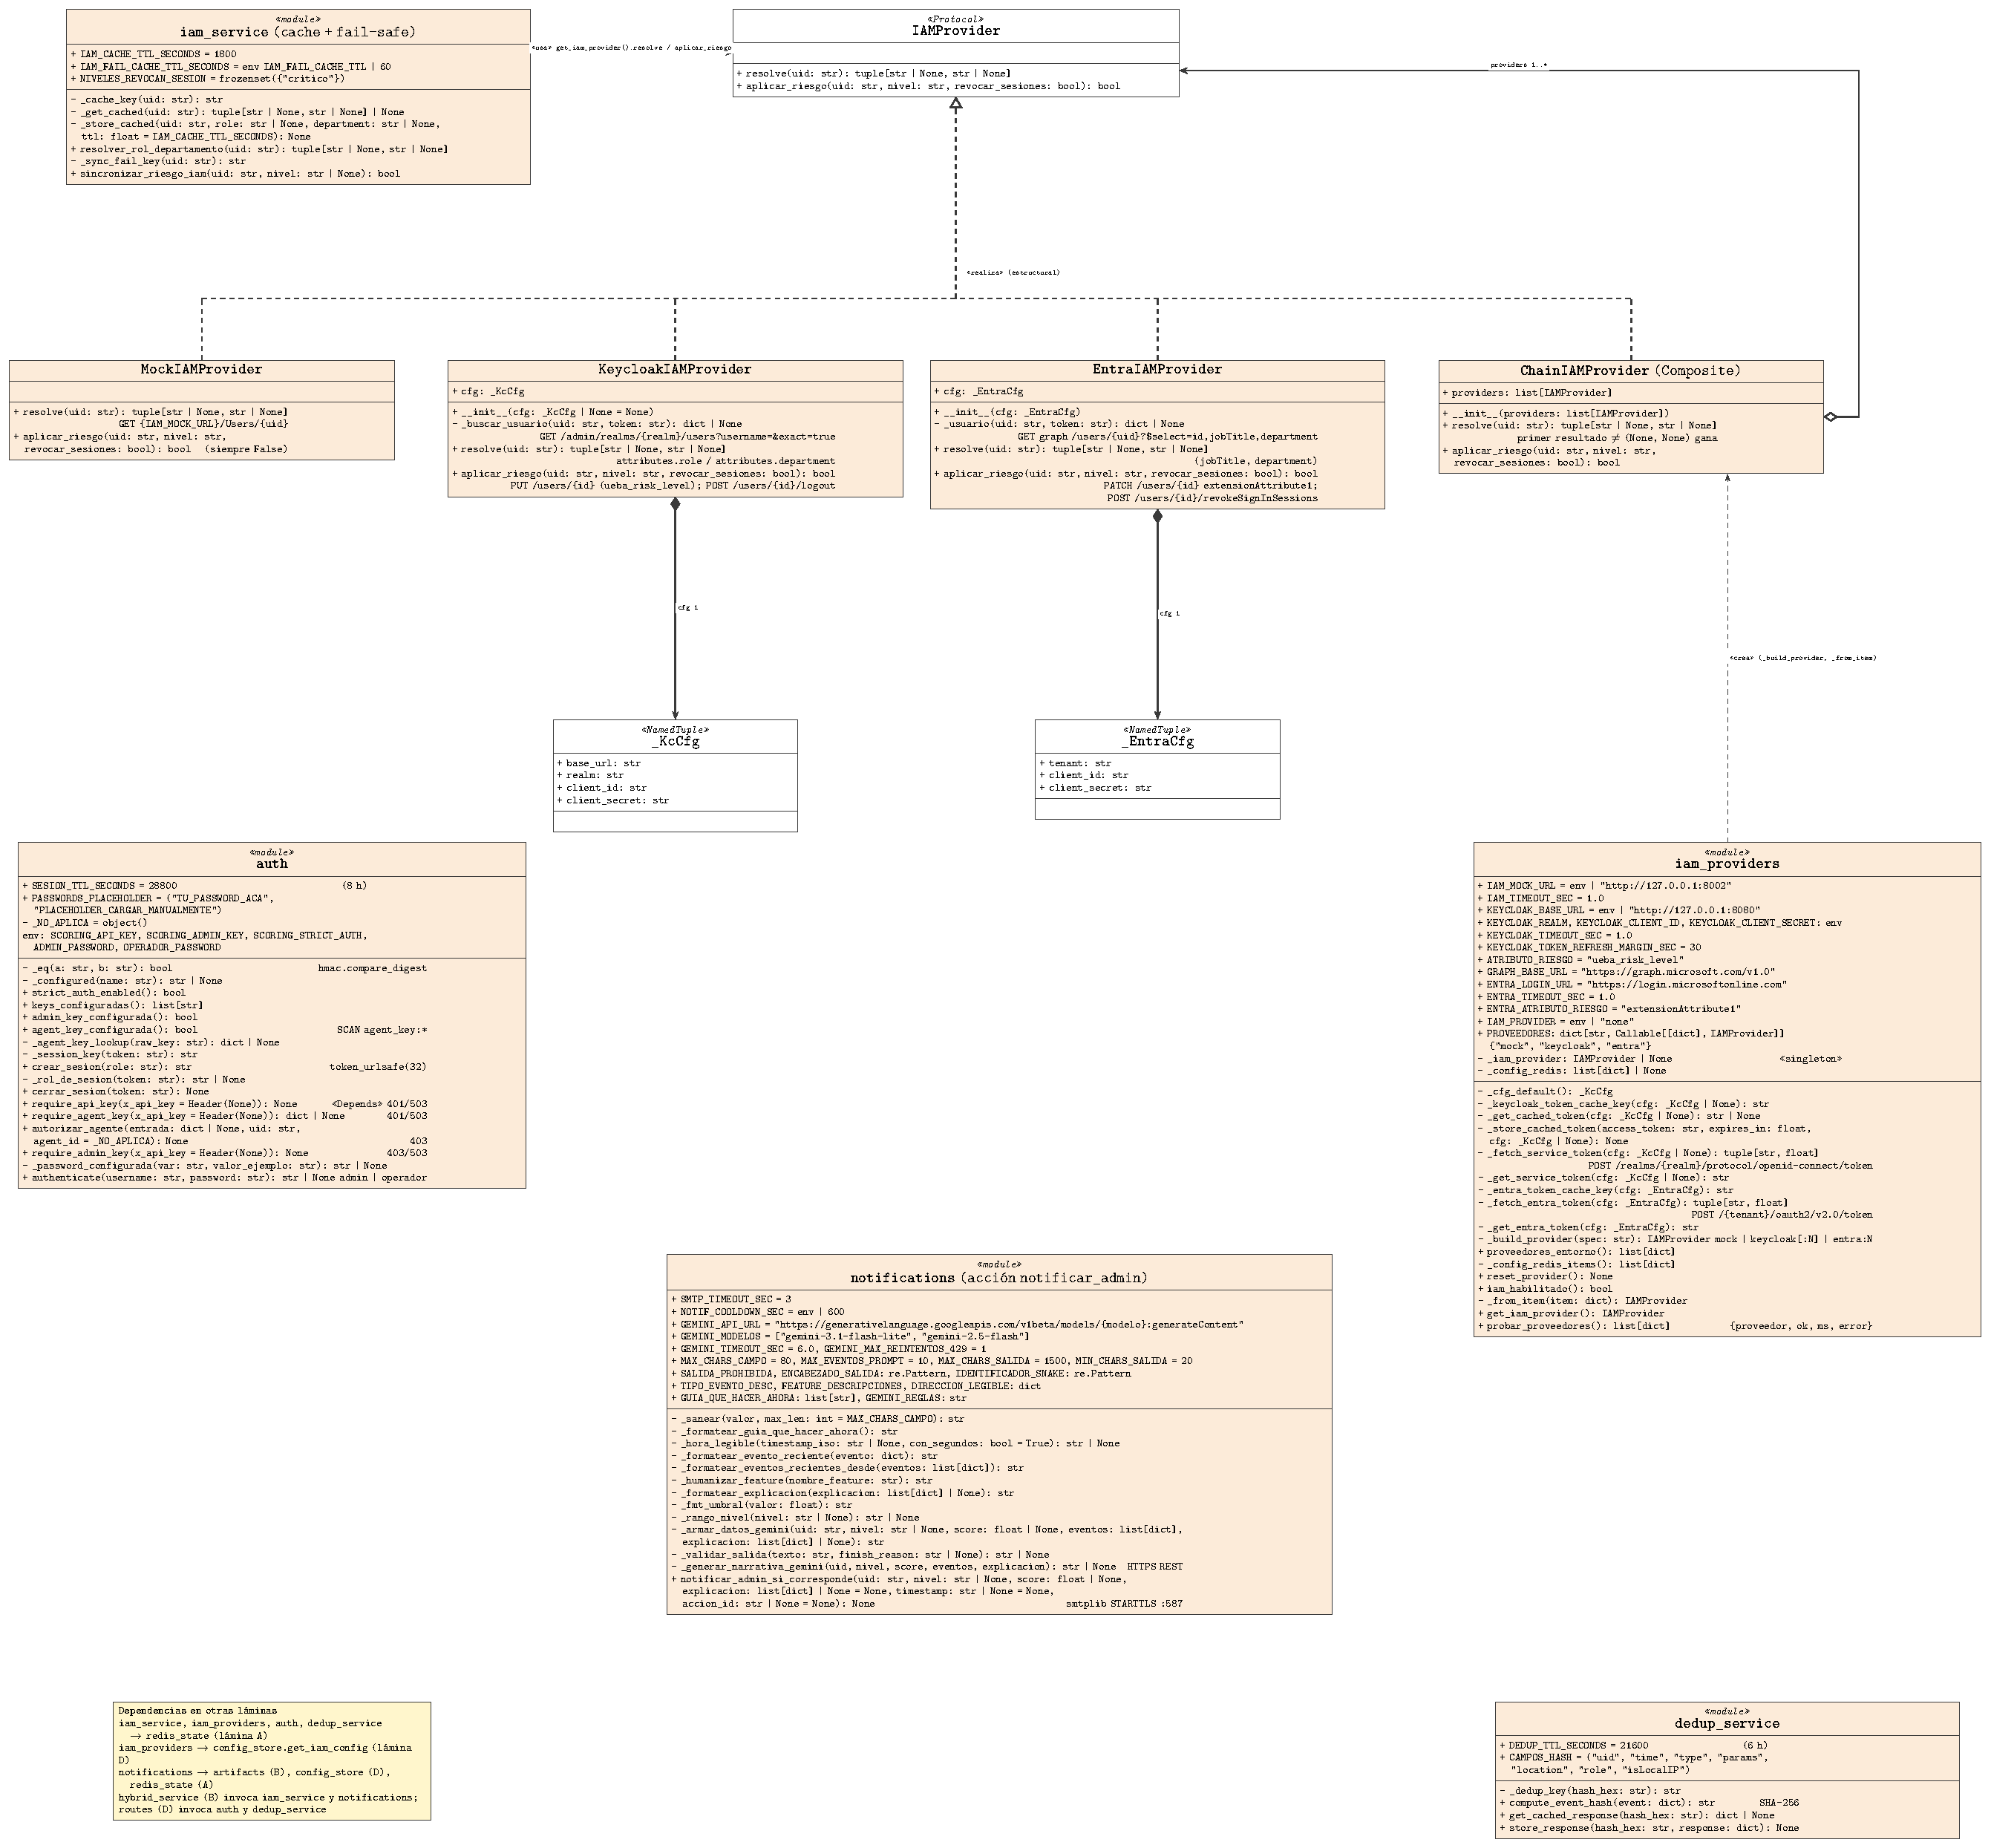
\includegraphics[trim=0bp 0bp 643.63bp 0bp, clip, width=\textwidth, height=0.84\textheight, keepaspectratio]{images/diagramas/uml/04c_clases_api_iam_auth.pdf}
    \caption{Diagrama de clases de la API PDP: proveedores de identidad y autenticación, versión completa (mitad izquierda)}
    \label{fig:anexo-clases-iam-izq}
    {\small Fuente: elaboración propia.\par}
\end{figure}
\clearpage

\begin{figure}[p]
    \centering
    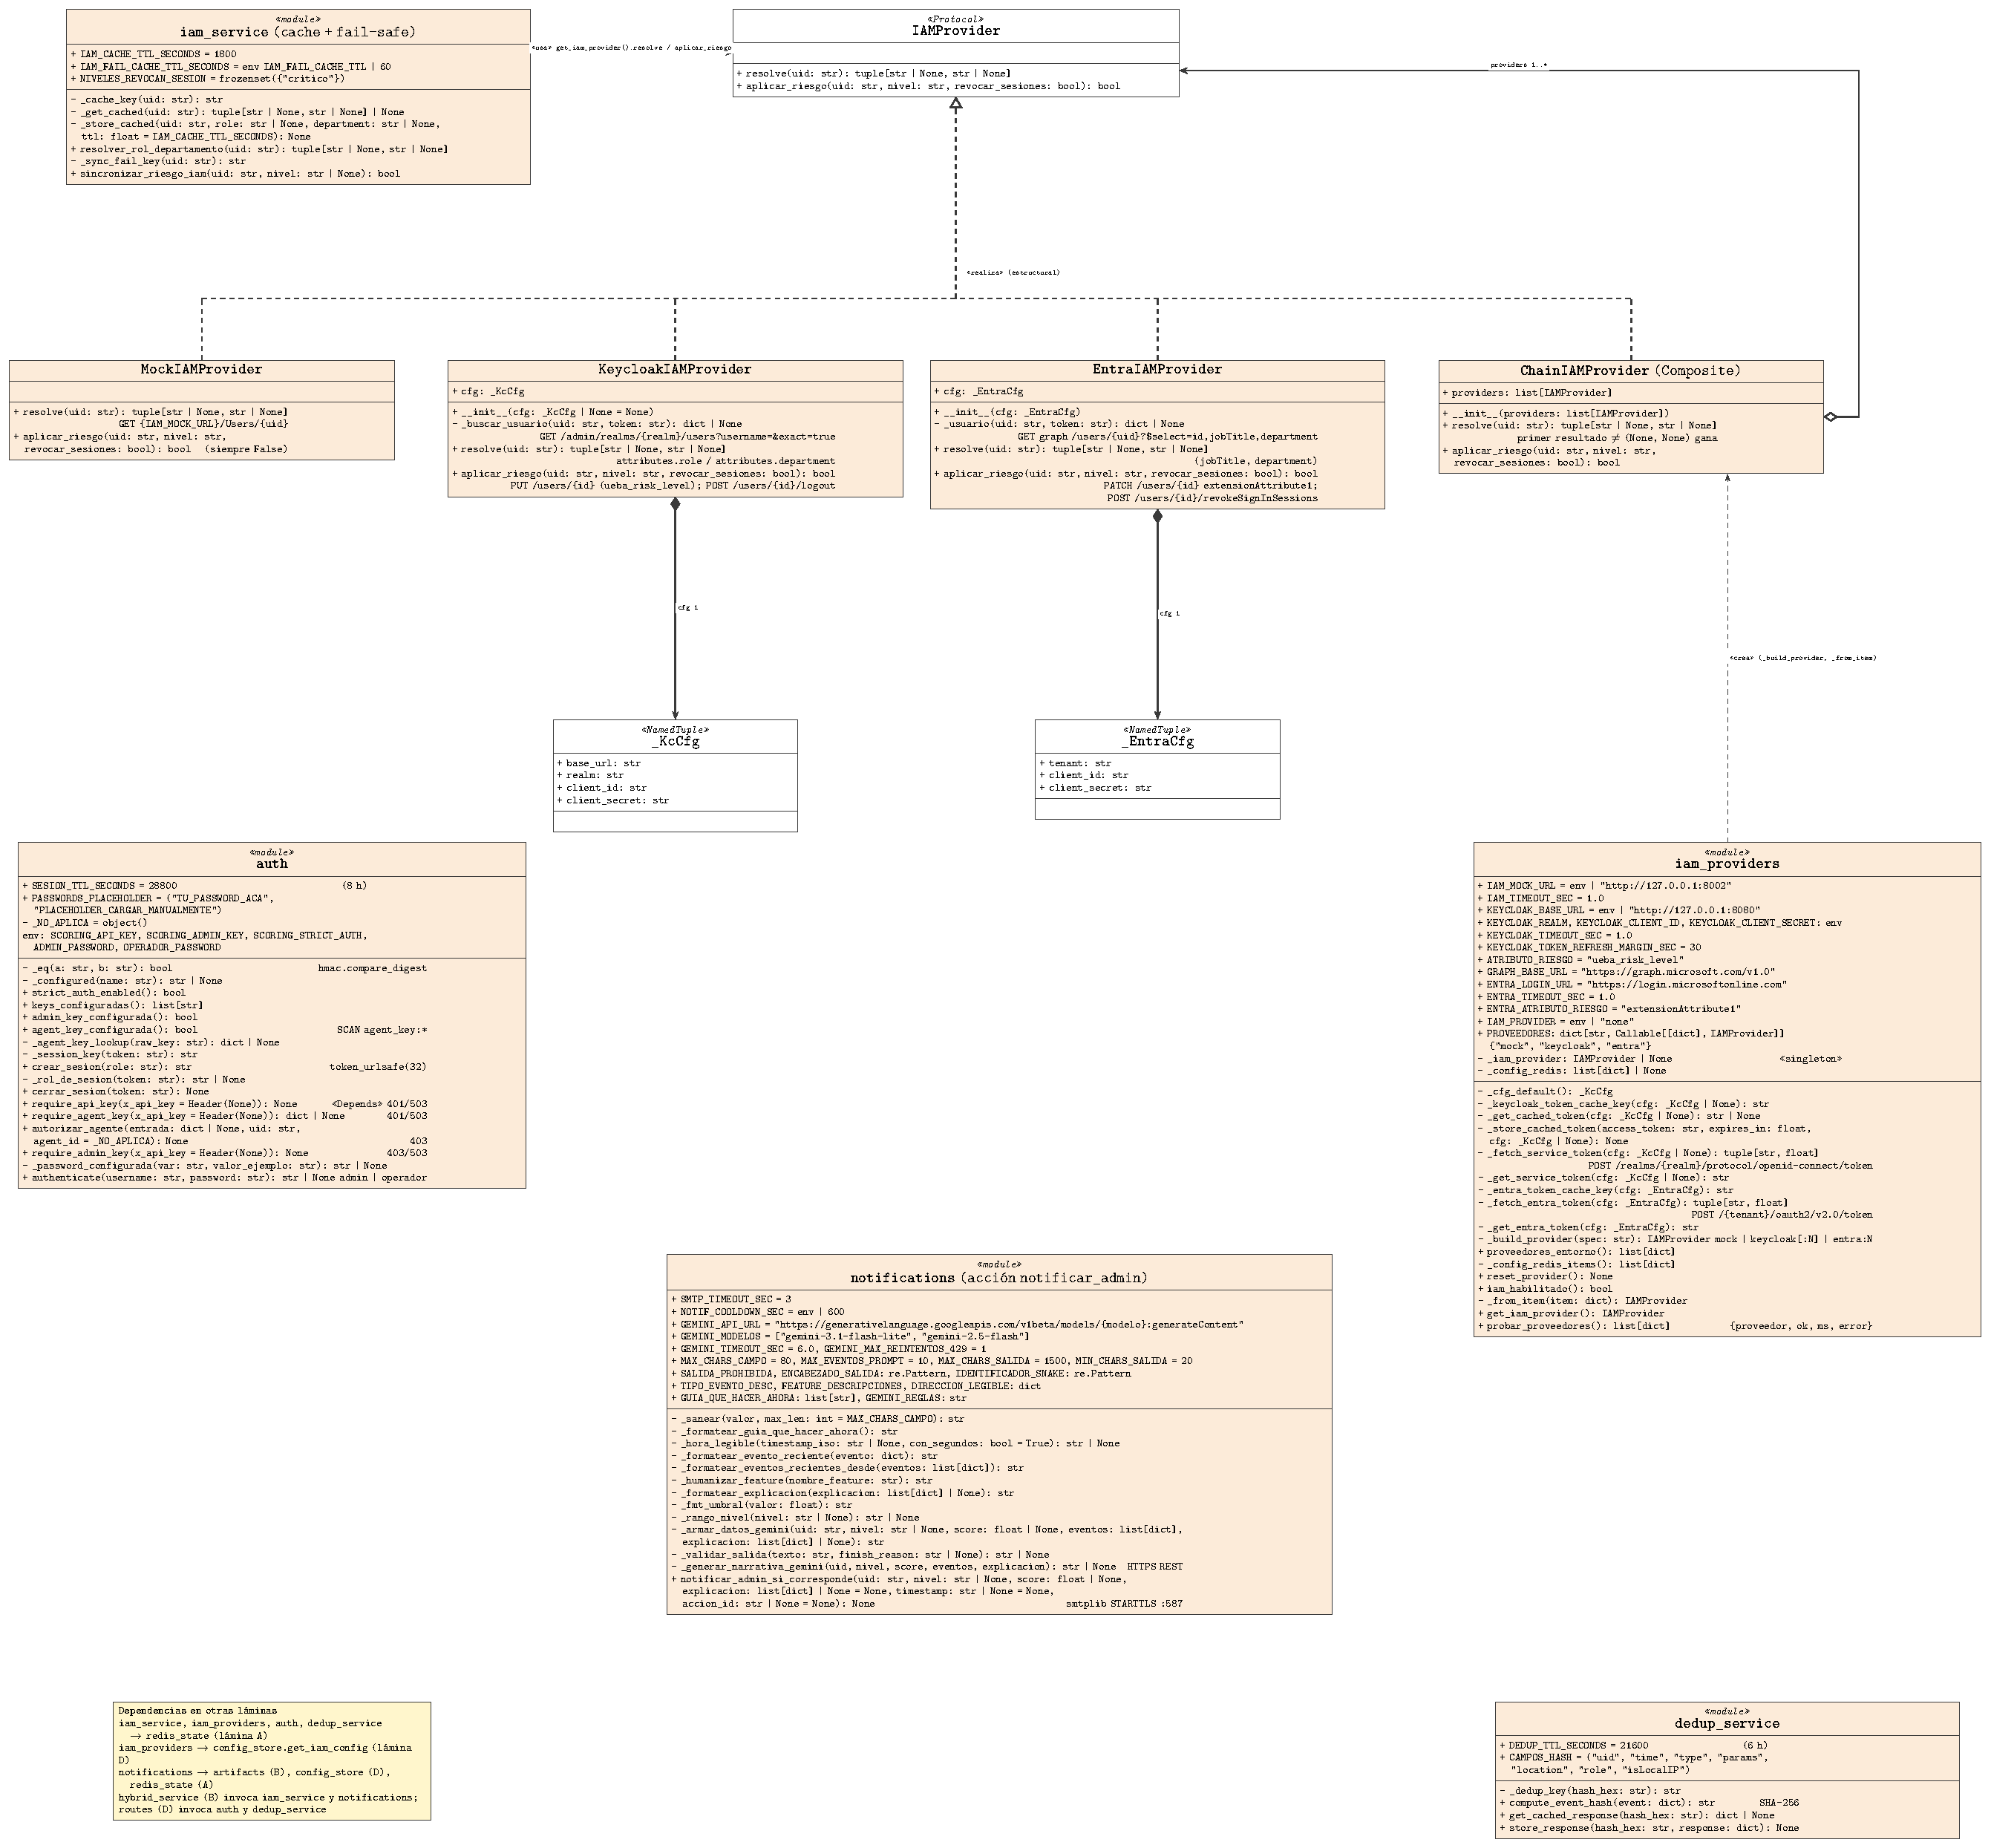
\includegraphics[trim=643.63bp 0bp 0bp 0bp, clip, width=\textwidth, height=0.84\textheight, keepaspectratio]{images/diagramas/uml/04c_clases_api_iam_auth.pdf}
    \caption{Diagrama de clases de la API PDP: proveedores de identidad y autenticación, versión completa (mitad derecha)}
    \label{fig:anexo-clases-iam-der}
    {\small Fuente: elaboración propia.\par}
\end{figure}
\clearpage

\begin{figure}[p]
    \centering
    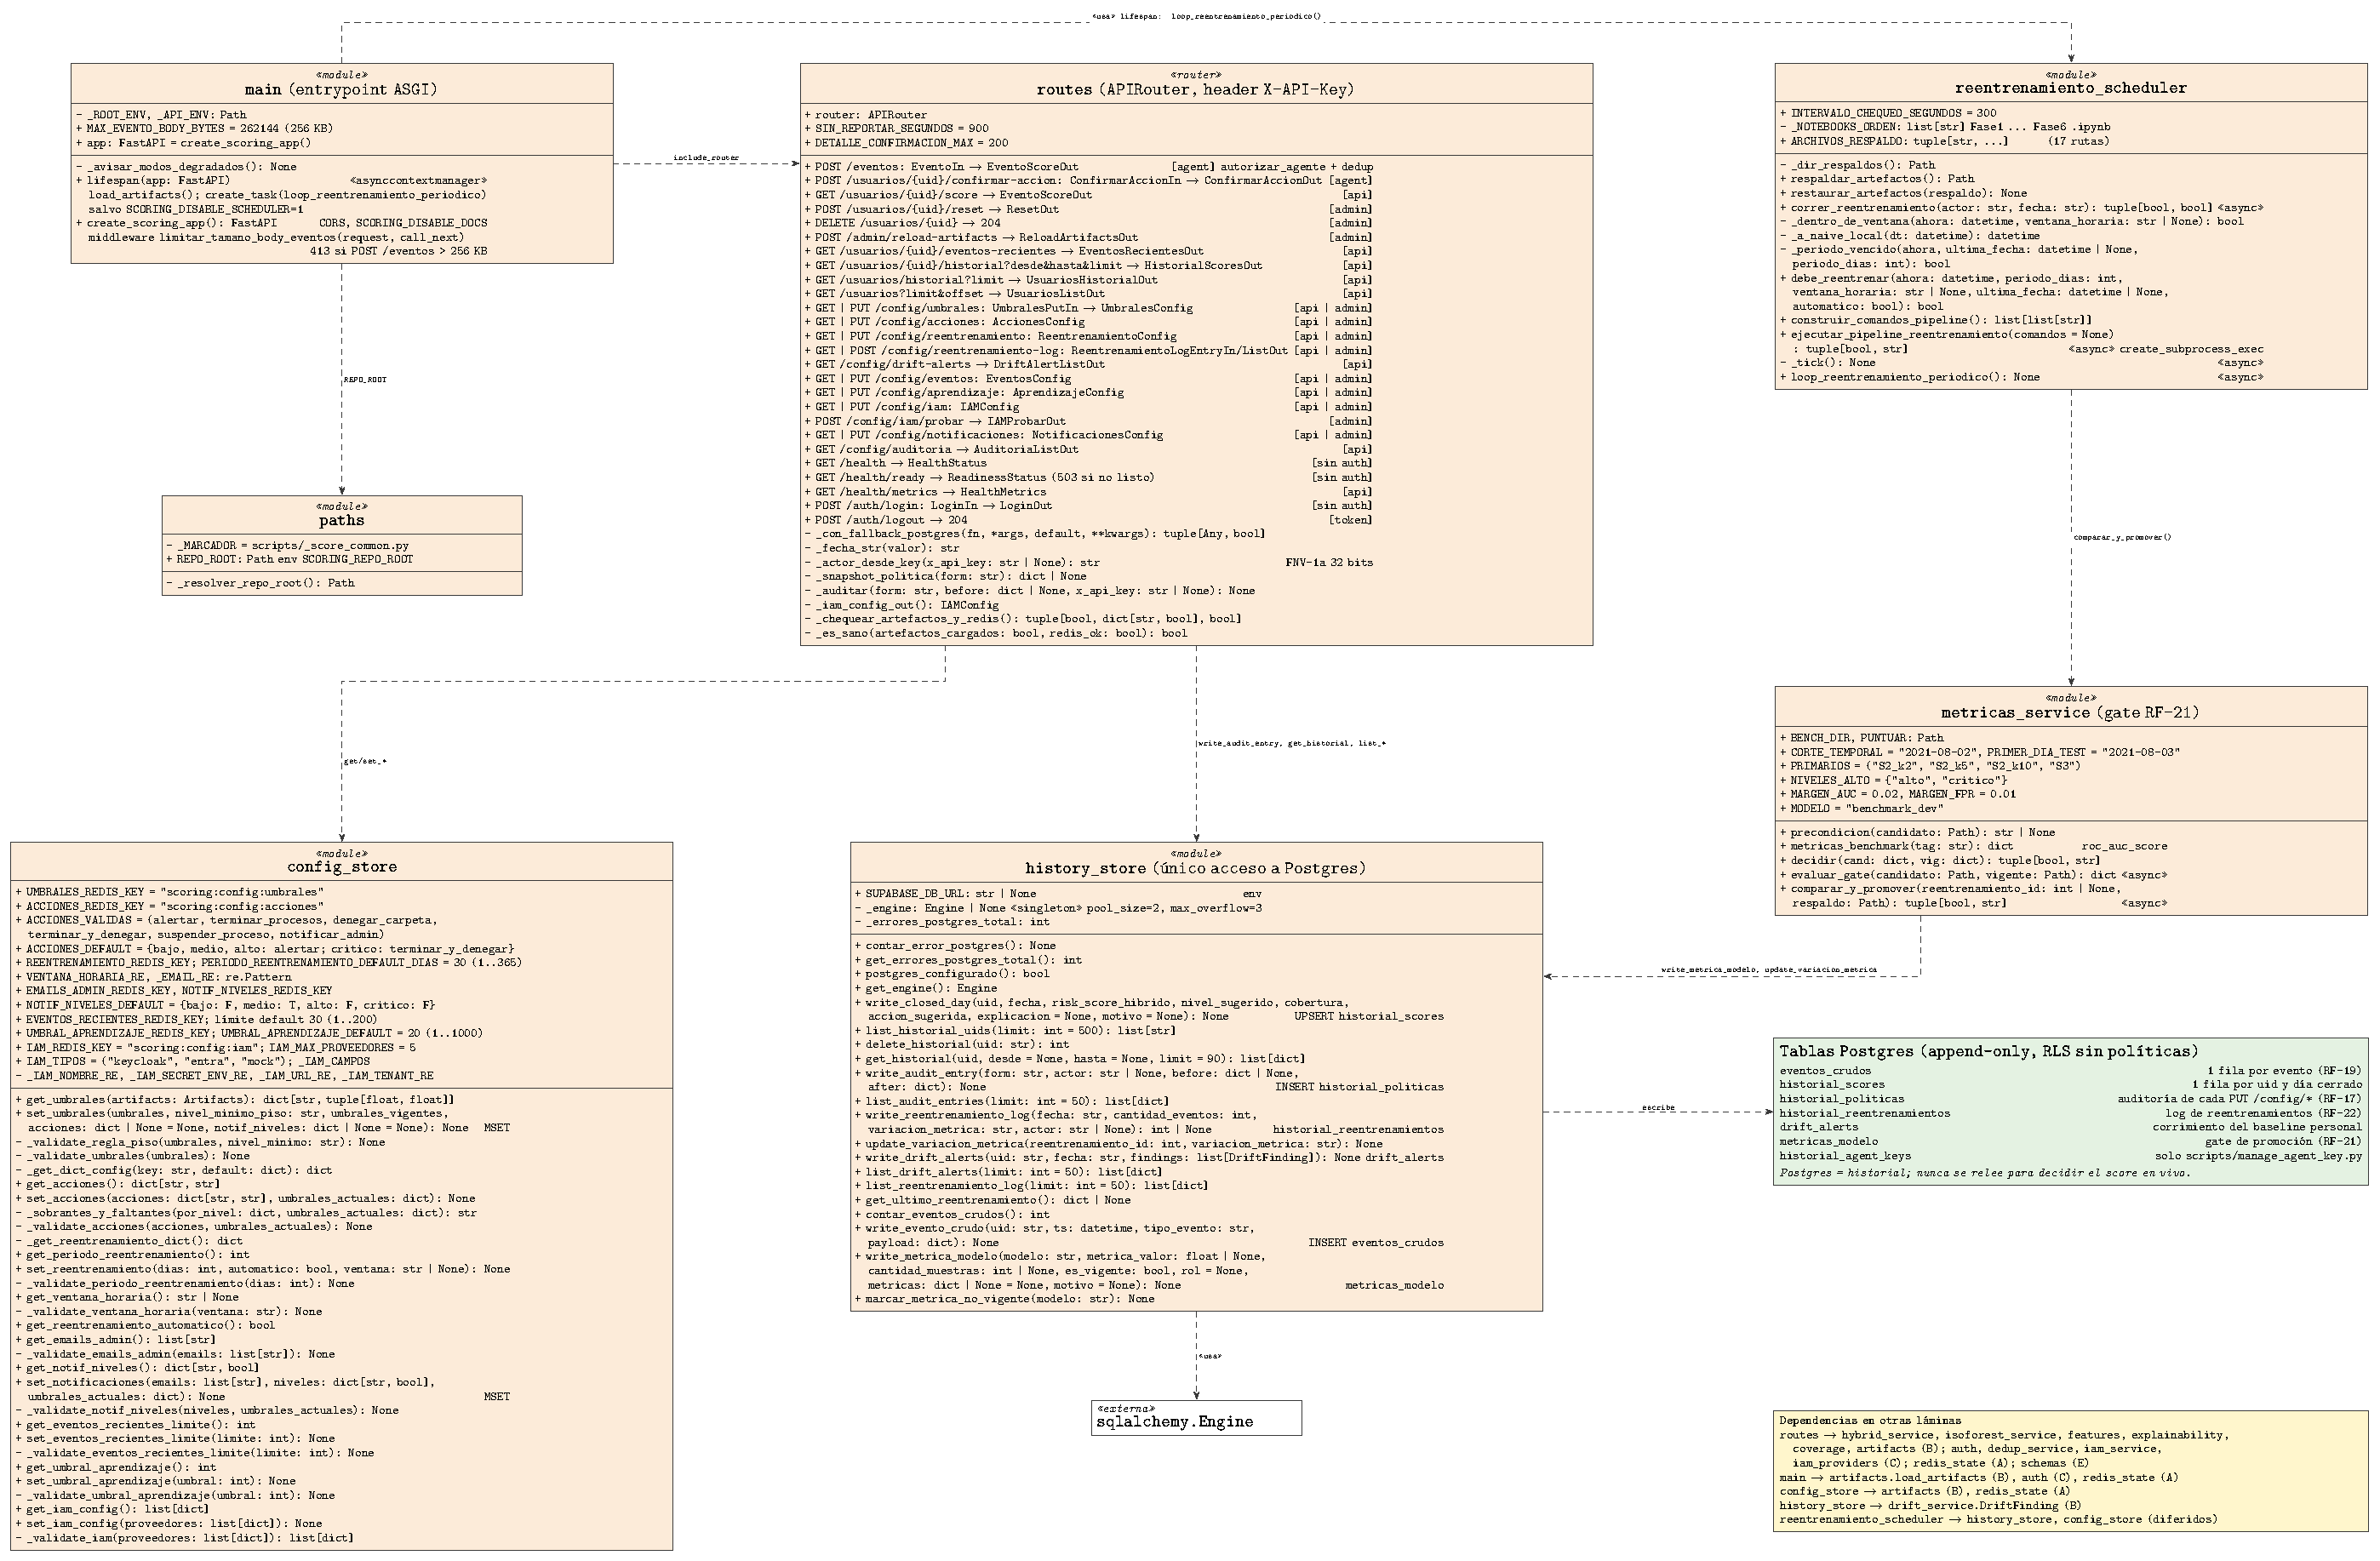
\includegraphics[trim=0bp 0bp 670.97bp 0bp, clip, width=\textwidth, height=0.84\textheight, keepaspectratio]{images/diagramas/uml/04d_clases_api_persistencia_config.pdf}
    \caption{Diagrama de clases de la API PDP: rutas, persistencia, configuración y reentrenamiento, versión completa (mitad izquierda)}
    \label{fig:anexo-clases-persistencia-izq}
    {\small Fuente: elaboración propia.\par}
\end{figure}
\clearpage

\begin{figure}[p]
    \centering
    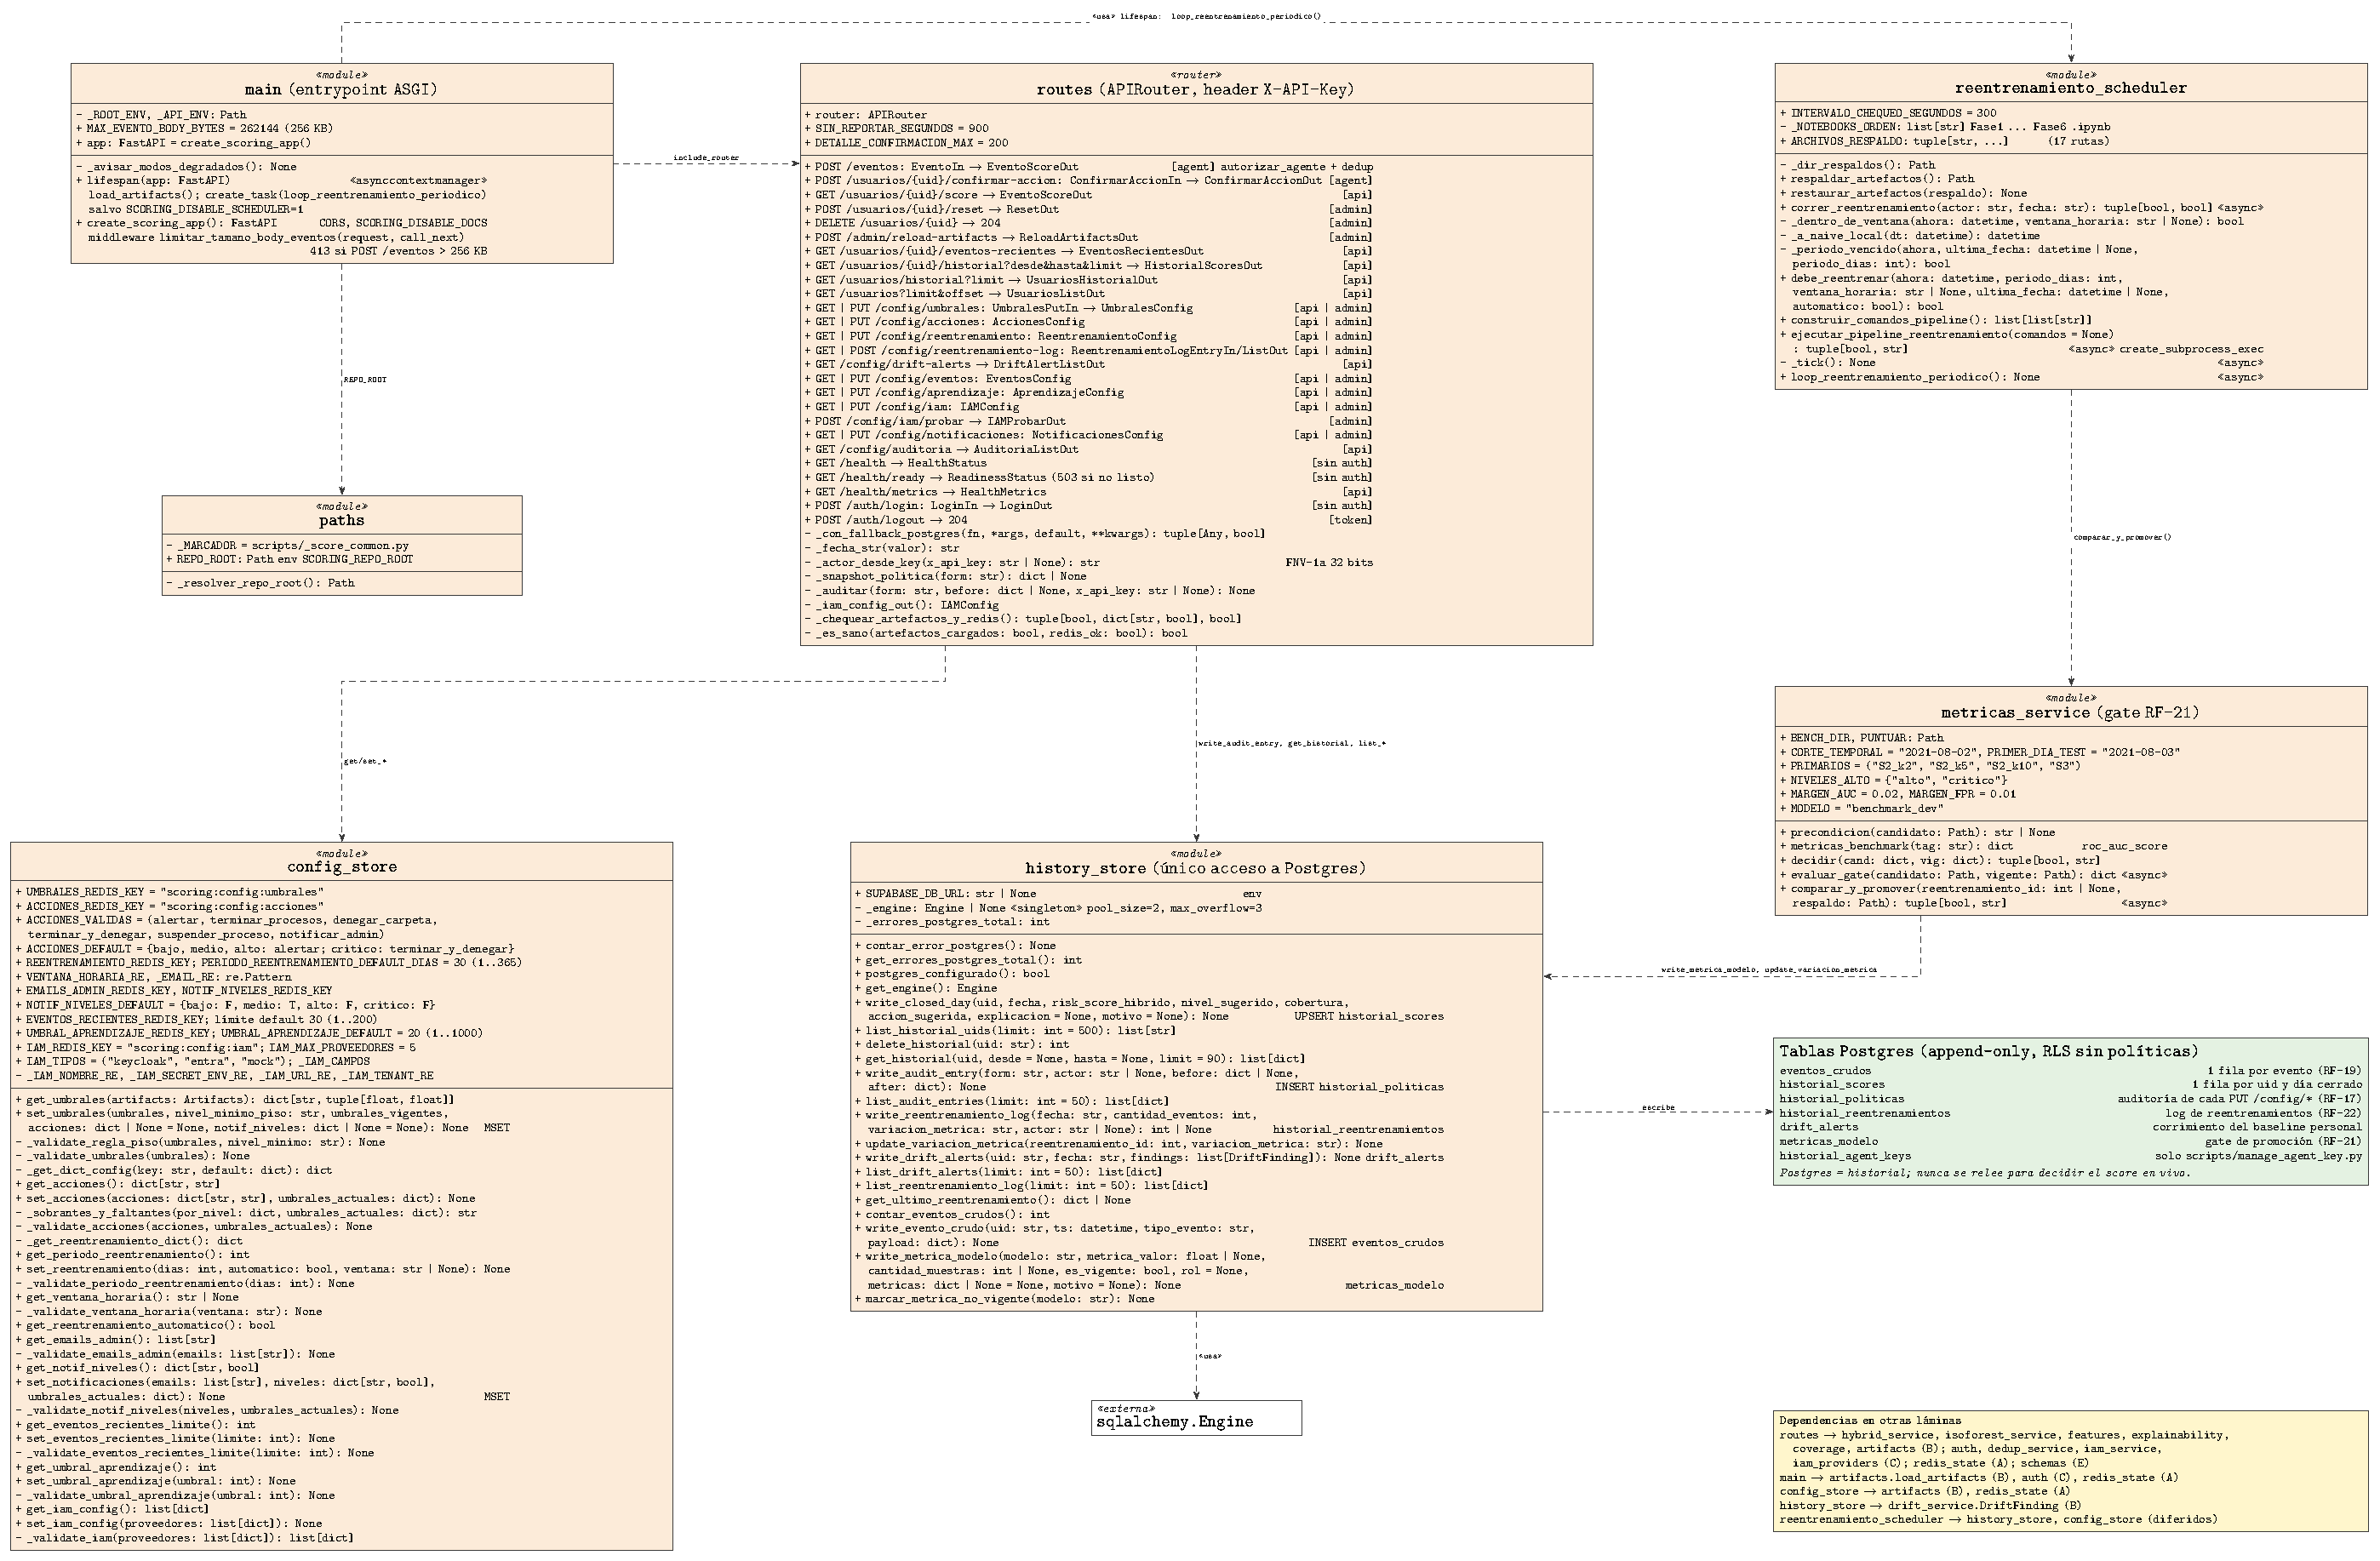
\includegraphics[trim=670.97bp 0bp 0bp 0bp, clip, width=\textwidth, height=0.84\textheight, keepaspectratio]{images/diagramas/uml/04d_clases_api_persistencia_config.pdf}
    \caption{Diagrama de clases de la API PDP: rutas, persistencia, configuración y reentrenamiento, versión completa (mitad derecha)}
    \label{fig:anexo-clases-persistencia-der}
    {\small Fuente: elaboración propia.\par}
\end{figure}
\clearpage

\begin{figure}[p]
    \centering
    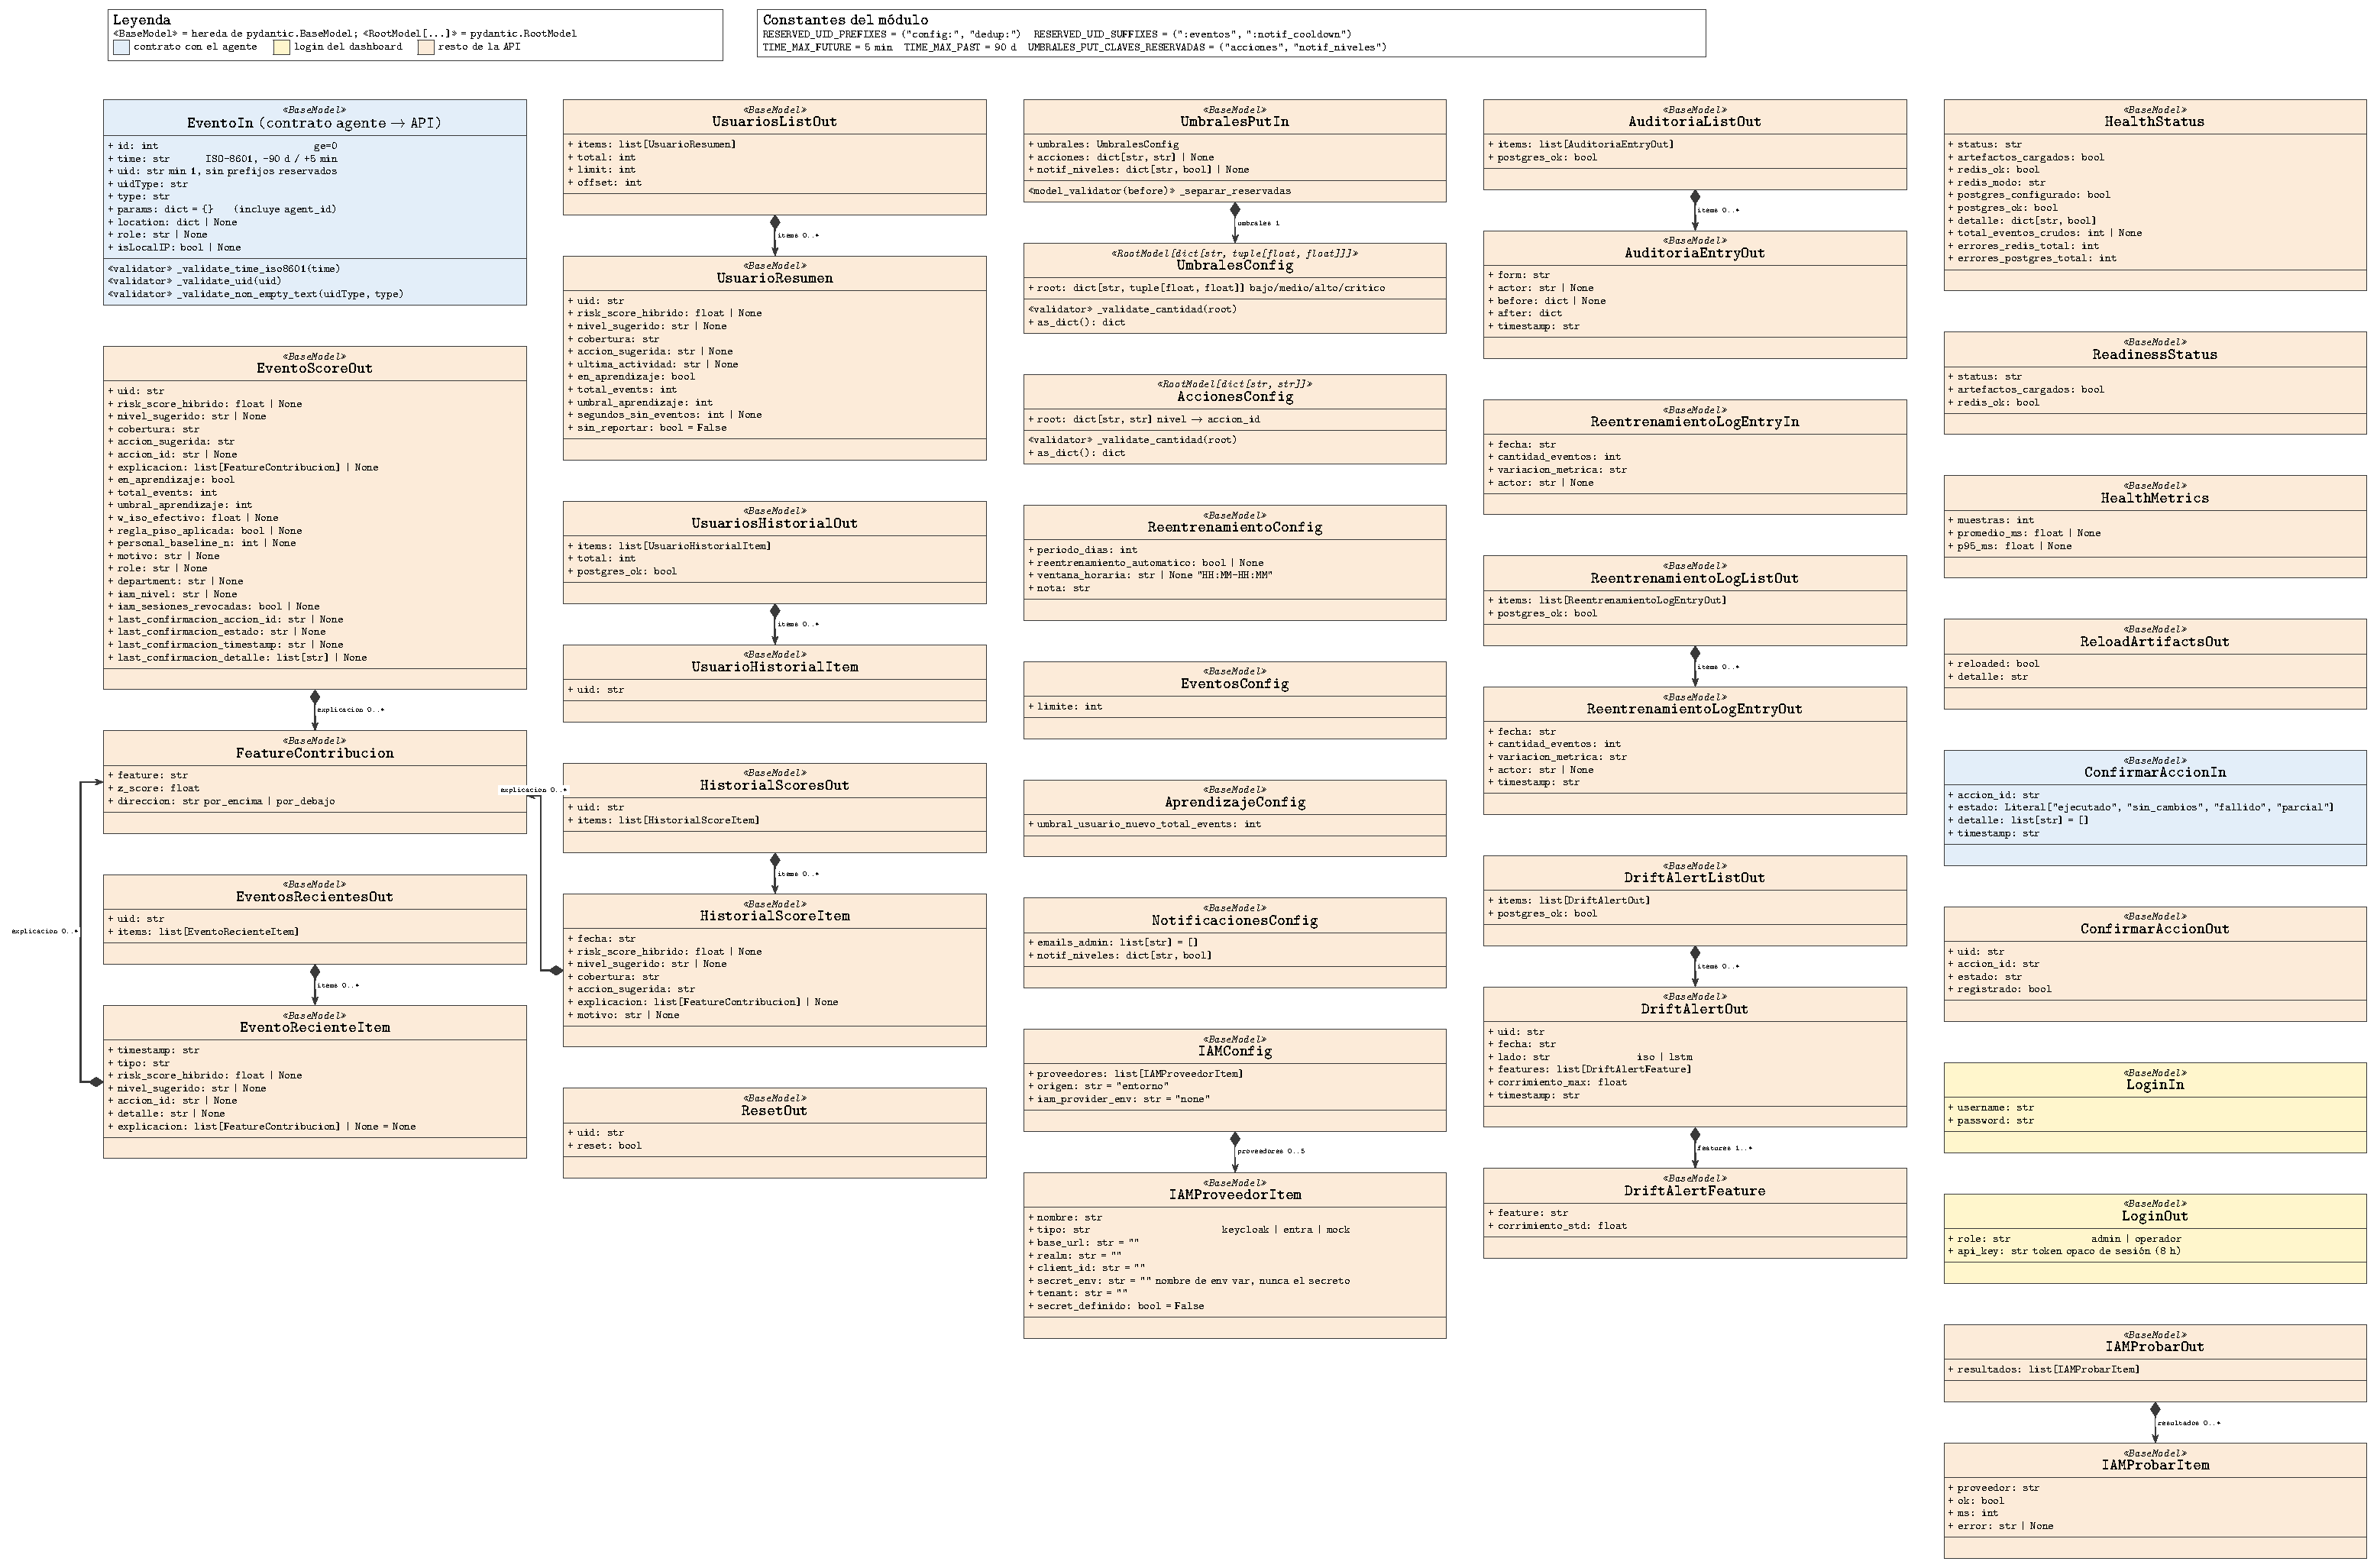
\includegraphics[trim=0bp 0bp 746.78bp 0bp, clip, width=\textwidth, height=0.84\textheight, keepaspectratio]{images/diagramas/uml/04e_clases_api_schemas.pdf}
    \caption{Diagrama de clases de la API PDP: esquemas HTTP, versión completa (mitad izquierda)}
    \label{fig:anexo-clases-schemas-izq}
    {\small Fuente: elaboración propia.\par}
\end{figure}
\clearpage

\begin{figure}[p]
    \centering
    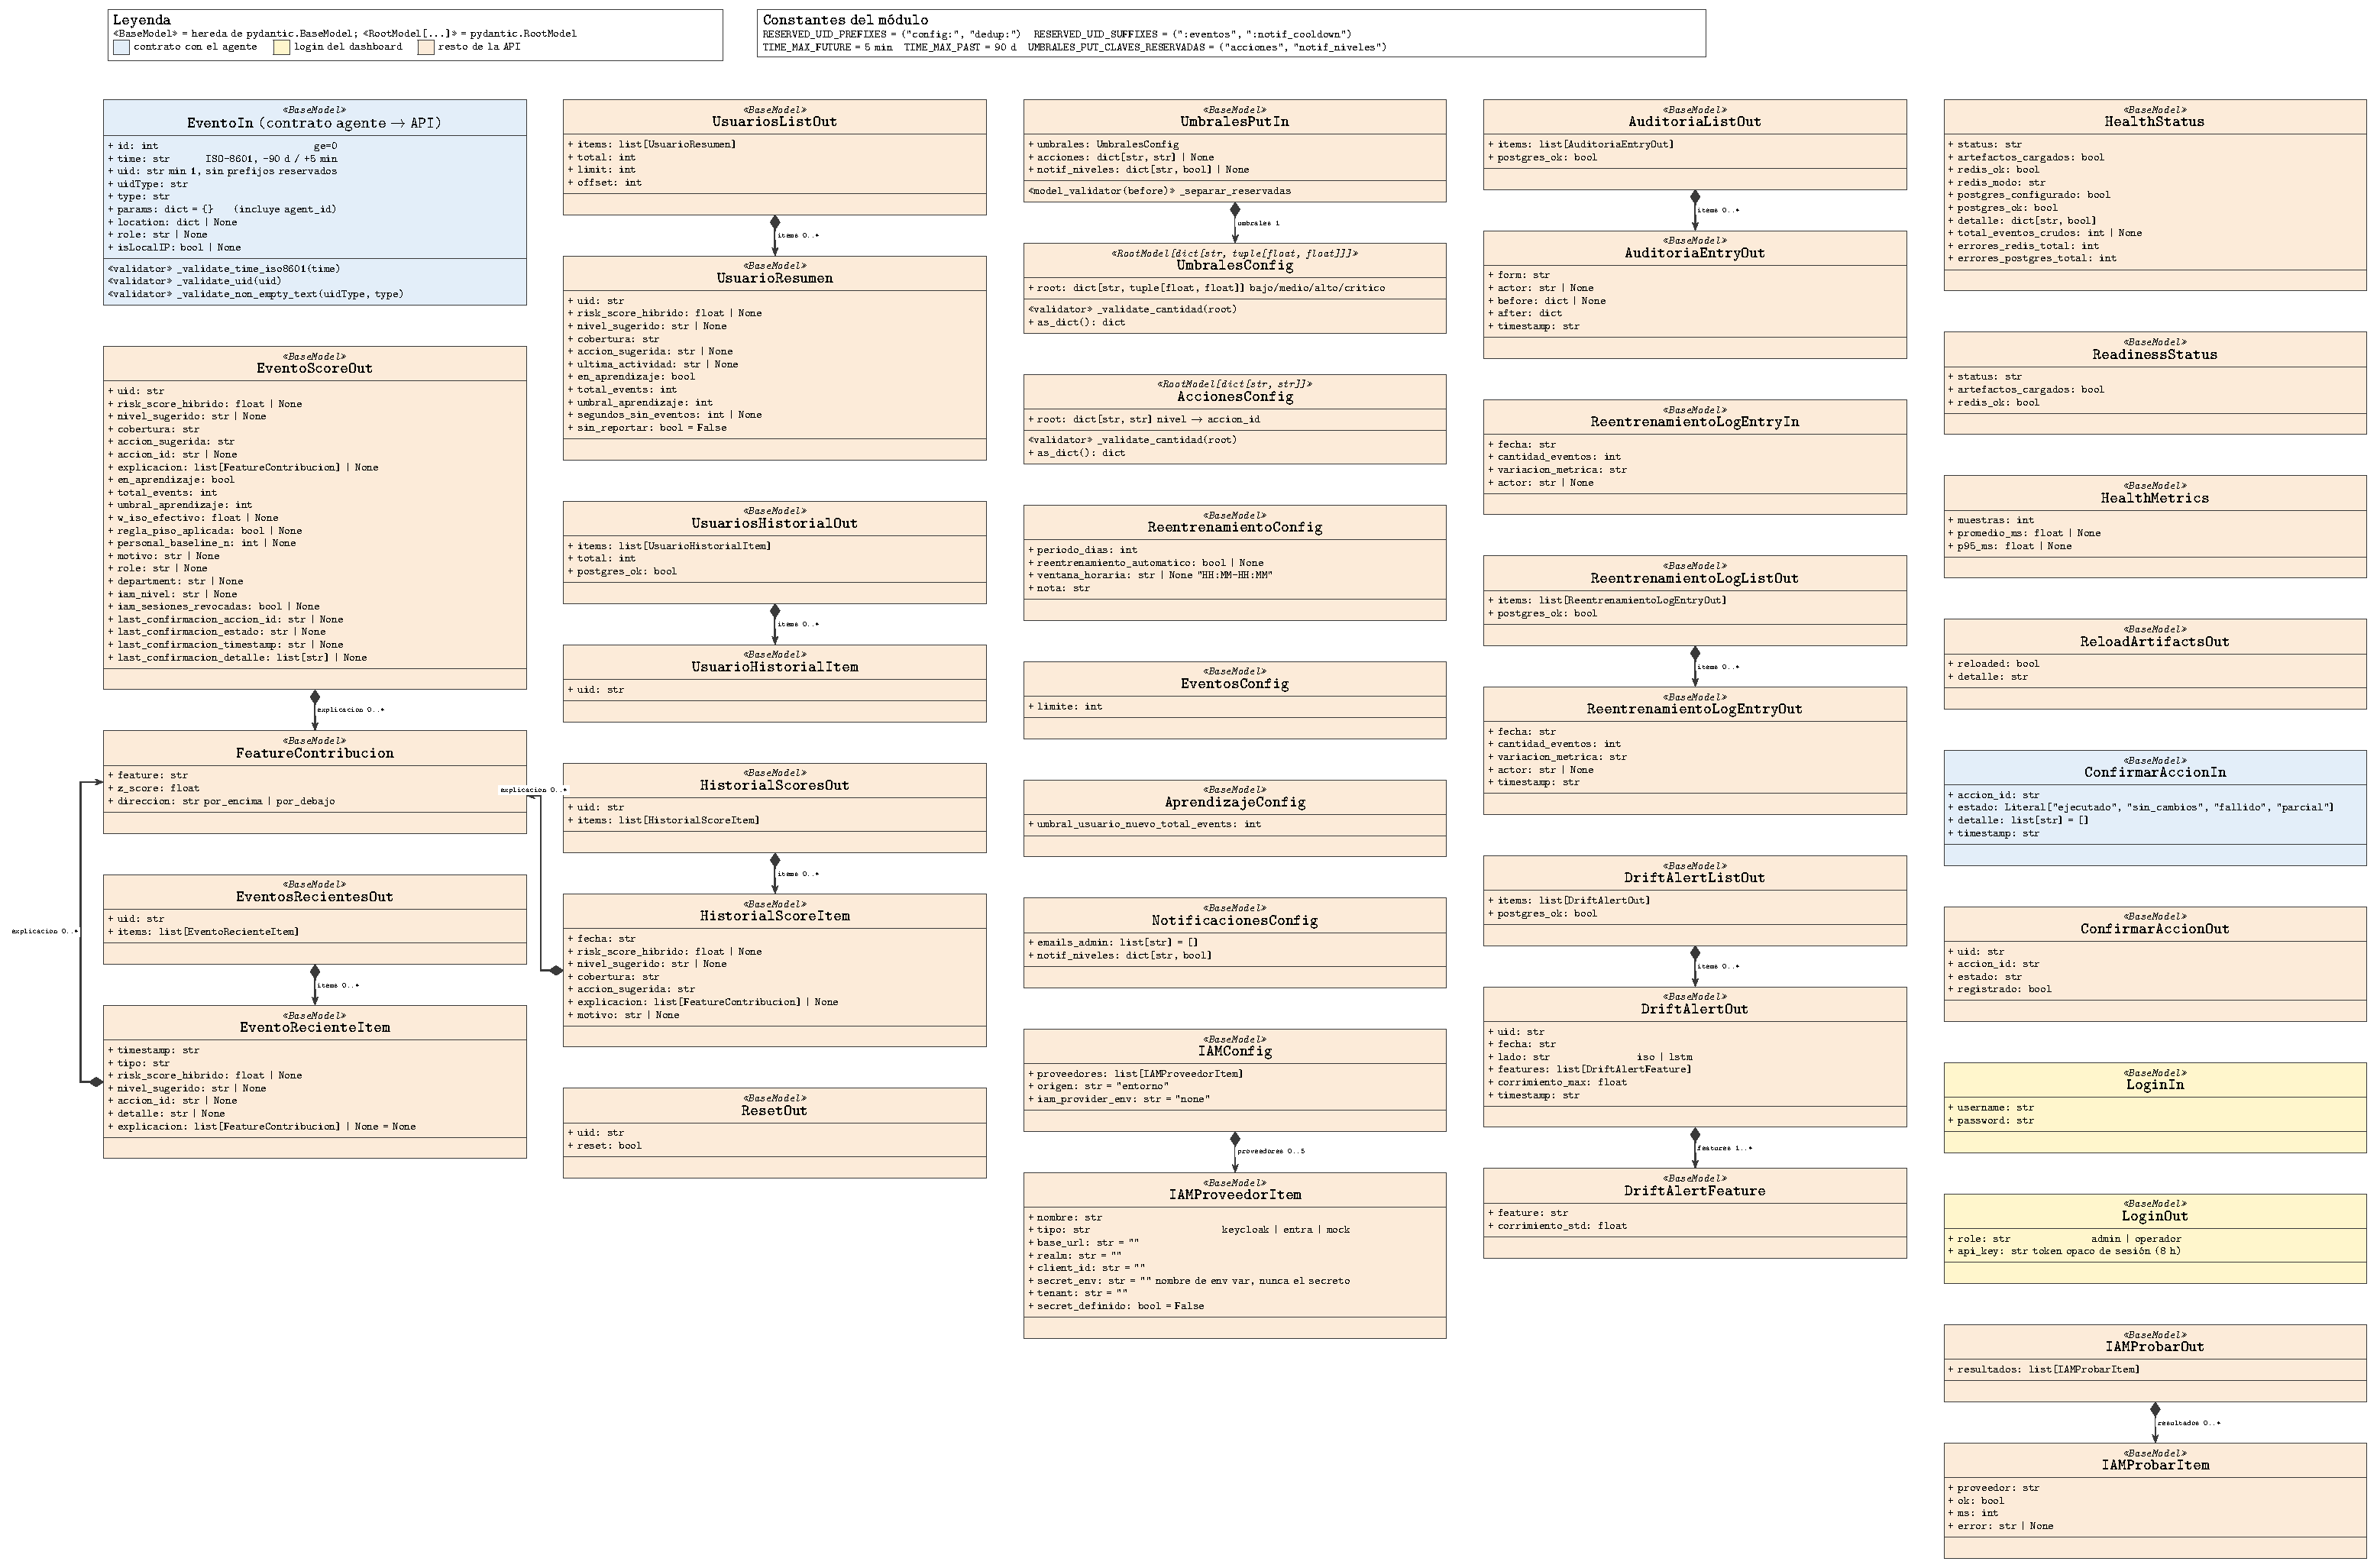
\includegraphics[trim=746.78bp 0bp 0bp 0bp, clip, width=\textwidth, height=0.84\textheight, keepaspectratio]{images/diagramas/uml/04e_clases_api_schemas.pdf}
    \caption{Diagrama de clases de la API PDP: esquemas HTTP, versión completa (mitad derecha)}
    \label{fig:anexo-clases-schemas-der}
    {\small Fuente: elaboración propia.\par}
\end{figure}
\clearpage
